\documentclass[journal]{IEEEtran}
\IEEEoverridecommandlockouts

%%%%%%%%%%%%%%%%%%%%%%%%%%%%%%%%%%%%%%
%%%%%%%% PACCHETTI PRINCIPALI %%%%%%%%
%%%%%%%%%%%%%%%%%%%%%%%%%%%%%%%%%%%%%%
\usepackage{fancyhdr}
\usepackage{graphicx}
\usepackage[italian]{babel}
\usepackage[utf8]{inputenc}
\usepackage{color}
\usepackage{hyperref}
\usepackage{wrapfig}
\usepackage{array}
\usepackage{multirow}
\usepackage{adjustbox}
\usepackage{nccmath}
\usepackage{subfigure}
\usepackage{amsfonts,latexsym}
\usepackage{enumerate}
\usepackage{booktabs}
\usepackage{float}
\usepackage{threeparttable}
\usepackage{array,colortbl}
\usepackage{ifpdf}
\usepackage{rotating}
\usepackage{cite}
\usepackage{stfloats}
\usepackage{url}
\usepackage{listings}
\usepackage{soul}

%%%%%%%%%%%%%%%%%%%%%%%%%%%%%%%%%%%%
%%% CREA E SCRIVI ALCUNI COMANDI %%%
%%%%%%%%%%%%%%%%%%%%%%%%%%%%%%%%%%%%
\newcolumntype{P}[1]{>{\centering\arraybackslash}p{#1}}  %% Viene creato un nuovo tipo di colonna denominata P.

% correggere la sillabazione errata qui
\hyphenation{op-tical net-works semi-conduc-tor} %% Con questo comando si specifica come separare correttamente le sillabe nel caso in cui una parola si trovi in due diverse righe di testo

\graphicspath{ {./img/} }  %%Percorso dove si trovano le immagini, se è vuoto indica che le immagini sono all'interno della stessa cartella che contiene il file .tex


%%%%%%%%%%%%%%%%%%%%%%%%%%%%%%%%%%%%%%%%%%%%%%%%
%%% INTESTAZIONE DELLE PAGINE TIPO UNICAFAM %%%%
%%%%%%%%%%%%%%%%%%%%%%%%%%%%%%%%%%%%%%%%%%%%%%%%
\newcommand{\MYhead}{\smash{\scriptsize
\hfil\parbox[t][\height][t]{\textwidth}{\centering
\begin{picture}(0,0) \put(-30,-13){
\includegraphics[width=30mm]{logoUnisalento.jpg}} \end{picture} \hspace{6.4cm}
INGEGNERIA INFORMATICA \\
\hspace{5.2cm} DIPARTIMENTO DI INGEGNERIA DELL'INNOVAZIONE \hspace{3cm} \\
\underline{\hspace{ \textwidth}}}\hfil\hbox{}}}
\makeatletter

% normal pages
\def\ps@headings{%
\def\@oddhead{\MYhead}%
\def\@evenhead{\MYhead}}%

% title page
\def\ps@IEEEtitlepagestyle{%
\def\@oddhead{\MYhead}%
\def\@evenhead{\MYhead}}%
\makeatother

% make changes take effect
\pagestyle{headings}

% adjust as needed
\addtolength{\footskip}{0\baselineskip}
\addtolength{\textheight}{-1\baselineskip}

%define colors for code language
\definecolor{codegreen}{rgb}{0,0.7,0.3}
\definecolor{codegray}{rgb}{0,0,0}
\definecolor{codepurple}{rgb}{0.58,0,0.82}
\definecolor{backcolour}{rgb}{0.95,0.95,0.95}
\definecolor{keywordcolor}{rgb}{0.8,0.3,0}

\lstdefinestyle{mystyle}{
    backgroundcolor=\color{backcolour},   
    commentstyle=\color{codegreen},
    keywordstyle=\color{keywordcolor},
    numberstyle=\tiny\color{codegray},
    stringstyle=\color{codepurple},
    basicstyle=\ttfamily\footnotesize,
    breakatwhitespace=false,         
    breaklines=true,                 
    captionpos=b,                    
    keepspaces=true,                 
    numbers=left,                    
    numbersep=5pt,                  
    showspaces=false,                
    showstringspaces=false,
    showtabs=false,                  
    tabsize=4
}

\lstset{style=mystyle}



%%%%%%%%%%%%%%%%%%%%%%%%%%%%%%%%
%%%%% INIZIO DEL DOCUMENTO %%%%%
%%%%%%%%%%%%%%%%%%%%%%%%%%%%%%%%
\begin{document}



%%%%%%%%%%%%%%%%%%%%%%%%%%%%
%%% TITOLO DEL DOCUMENTO %%%
%%%%%%%%%%%%%%%%%%%%%%%%%%%%
\title{Pianificazione Automatica e \\sistemi di Supporto delle Decisioni}



%%%%%%%%%%%%%%%%%%%%%%%%%%
%%%%%%%%% AUTORE %%%%%%%%%
%%%%%%%%%%%%%%%%%%%%%%%%%%
\author{Matteo Aprile\\
				Professore: Giampaolo Ghiani, Enamuele Manni\\
        }
        
%scrive il titolo
\maketitle

%scrive l'indice
\tableofcontents
\underline{\hspace{ 80 mm }}



%%%%%%%%%%%%%%%%%%%%%%%%%%%%%
%%% SEZIONI DEL DOCUMENTO %%%
%%%%%%%%%%%%%%%%%%%%%%%%%%%%%
\section{Definizioni - 22/23.09.22}

Ci occuperemo di 2 tipi di scenari:
\begin{itemize}
	\item usare \hl{algoritmi a supporto delle decisioni}
	\item usare algoritmi che \hl{sostituiscono completamente l'uomo}
\end{itemize}


% Business Analytics
\subsection{Business Analytics}

Disciplina che utilizza dati, statistiche, modelli matematici per \hl{aiutare a prendere delle decisioni in base a dei dati}.

Possiamo racchiudere i suoi \hl{passaggi} in:
\begin{enumerate}
	\item \hl{descriptive analytics}: capire \textbf{cosa sia successo nel passato} tramite i dati disponibili
	\item \hl{predictive analytics}: cercare di \textbf{fare delle previsioni} in base ai dati già disponibili
	\item \hl{prescriptive analytics}: \textbf{creare un piano di azione} per poter massimizzare il KPI (Key Performance Indicator)
\end{enumerate}

\begin{figure}[H]
\centering
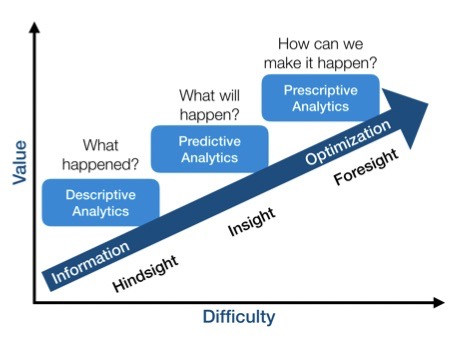
\includegraphics[scale=0.9]{businessAnalytics.jpeg}
\caption{Fasi della business analytics} 
\label{busana}
\end{figure}


% Decisioni
\subsection{Decisioni}

Rappresenta la \hl{scelta di un elemento tra più soluzioni} dopo aver ponderato le opzioni.

Possiamo avere più casi d'uso:
\begin{itemize}
	\item \hl{simplest case}: abbiamo \textbf{poche alternative} quindi una semplice scelta
	\item \hl{multple criteria}: abbiamo \textbf{più metri di paragone} delle performance, quindi si dovranno tenere in conto:
	
	\begin{itemize}
		\item \textbf{soluzioni migliori} di altre (dette di Pareto)
		\item \textbf{vincoli} dovuti dai clienti o da casi logistici da gestire (es: spedizioni)
		\item ottimizzazioni matematiche
		\item \textbf{conflitti tra i vincoli}
	\end{itemize}
	
	\item \hl{incertezze e rischi}: 
	
	\begin{itemize}
		\item \textbf{decisioni operative}: di \textbf{breve periodo}  \textbf{reversibili} e \textbf{limitate} a "n" persone del team
		
		\item \textbf{decisioni tattiche}: \textbf{coinvolge una parte dell'organizzazione} per un medio periodo
		
		\item \textbf{decisioni strategiche}: di \textbf{lungo periodo}  \textbf{non reversibili} e \textbf{coinvolgono denaro}
		
		\item \textbf{decisioni strutturate}: hanno una \textbf{procedura di risoluzione specifica}
		
		\item \textbf{decisioni non strutturate}: richiedono \textbf{creatività} ed \textbf{esperienza} in un  dato settore
	\end{itemize}
\end{itemize}

\begin{figure}[H]
\centering
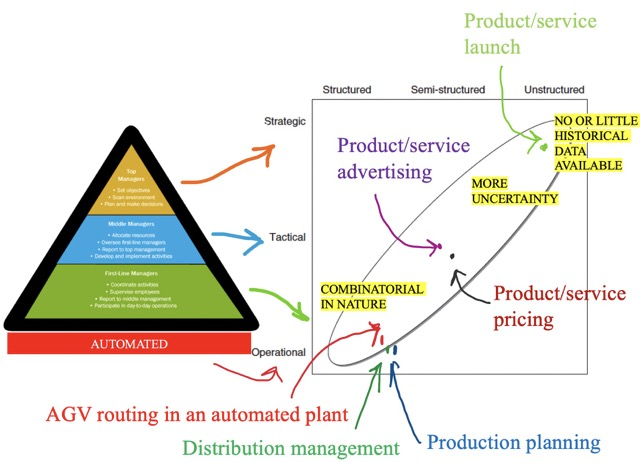
\includegraphics[scale=0.8]{dectax.jpeg}
\caption{Diagonale decisionale} 
\label{diadec}
\end{figure}


% Business Intelligence (BI)
\subsection{Business Intelligence (BI)}

Usato per indicare un \hl{sistema dedicato alla raccolta di dati e alla loro elaborazione} al fine di un reporting, infatti per "Inteligence" si intende investigazione.
Venivano \hl{usati su dati atomici} per avere delle conoscenze approfondite in un determinato business.


% Data visualization
\subsection{Data visualization}

Consiste nel \hl{prendere dati e plottare un grafico}, ma in realtà ora si ha una trattazione più metodologica, cioè se visualizzare in  modo statico o meno i dati.


% Decision Support Systems (DSS)
\subsection{Decision Support Systems (DSS)}

Si indicava un \hl{sistema computerizzato dotato di un sistema di "data managment"} per creare un modello di ottimizzazione, fornendo un feedback tramite un'interfaccia. Ora indica una varietà di sistemi per visualizzare i dati in larga misura o meno.


% Operations Research (OR)
\subsection{Operations Research (OR)}

\hl{Attivita organizzative per portare avanti un sistema logistico}. Per "research" si indica la ricerca delle operation per conseguire dei risultati, avremo come sottocategorie:
\begin{itemize}
	\item \textbf{ottimizzazione matematica}
	\item \textbf{queueing theory}: \textbf{studio matematico delle linee in attesa}  il limite è che funzionano solo con sistemi semplici e con richieste di servizio in ordine stocastico
	\item \textbf{simulazione}: per usarle è \textbf{necessario generare dei numeri randomici}  \textbf{quindi  inconveniente} (bisogna fare un analisi statistica dei risultati dalle quali si farà una \textbf{stima} 
	\item \textbf{game theory}: decisioni con \textbf{più players}
\end{itemize}


% Agents
\subsection{Agents}

È un \hl{sistema che si muove in un environment} (ambiente), ha dei \hl{sensori} tramite i quali percepisce alcuni aspetti del mondo che lo circonda quindi si crea una \hl{rappresentazione del mondo circostante} che può vedere. È capace di \hl{influenzare l'ambiente tramite degli attuatori} come ruote o braccia (intendiamo anche agenti software).

Possiamo classificarli come:
\begin{itemize}
	\item \hl{agenti autonomi}: se è concepito in modo tale che \textbf{tramite un'istruzione sintetica raggiunge un goal sviluppando le azioni per raggiungerlo}  In realtà può anche non essere una sequenza di azioni dato che \textbf{potrebbero esserci degli imprevisti}
	\item \hl{agenti intelligenti}: se
	\item \textbf{impara dall'esperienza}
	\item crea una \textbf{rappresentazione dell'ambiente} che lo circonda e \textbf{ci ragiona sopra} per un possibile risultato delle proprie azioni
	\item \textbf{si adatta ad un ambiente mutevole}
\end{itemize}

\begin{figure}[H]
\centering
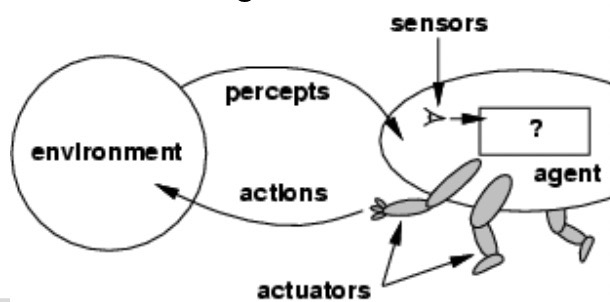
\includegraphics[scale=0.6]{agents.jpeg}
\caption{Schematizzazione di un agente e sue caratteristiche} 
\label{agente}
\end{figure}


% Artificial Intelligence (AI)
\subsection{Artificial Intelligence (AI)}

Comprende tante sottodiscipline:
\begin{itemize}
	\item \hl{automated reasoning}: legato alla \textbf{rappresentazione del mondo} e \textbf{come raggionare su di essa} ma anche calcolandone le probabilità
	\item \hl{automated planning}: usato in ambienti industriali
	\item \hl{automated learning}
	\item \hl{natural language processing}: \textbf{sviluppare agenti software} per fare sintesi di testi, scrivere automaticamente articoli, chat bot, ecc 
	\item \hl{perception}: visione artificiale
	\item \hl{manipuliation}: avere un \textbf{agente che può modificare l'agente} circostante
\end{itemize}


% Machine Learning (ML)
\subsection{Machine Learning (ML)}

Consiste nell'\hl{apprendimento automatico} e quindi lo sviluppo degli \hl{agenti che apprendo tramite la loro esperienza pregressa}. Ci sarà allora una fase di \hl{training}.
Una delle possibili \hl{architetture che permette di farlo sono le Neural Networks} prima avevano solo 2/3 neuroni, ora ne hanno vari strati il che fornisce delle prestazioni impressionanti


% Deep Leaning
\subsection{Deep Leaning}

Si basa sull'\hl{apprendimento automatico} con reti neurale tramite un gran numero di strati di neuroni.


% Data Mining (DM)
\subsection{Data Mining (DM)}

Usare metodi di Machine Learning per \hl{estrarre manualmente dei pattern dai dati}, cioè una \hl{regolarità o un trend}. È quindi la parte nobile del knowledge discovery in db, dato che i dati sono in genere disponibili su db o da altre piattaforme.

La \hl{sequenza} nella quale interviene è:
\begin{enumerate}
	\item \textbf{prendere} i dati
	\item trovare i vari \textbf{target}
	\item \textbf{preprocessare} i dati
	\item trasformare i dati tramite il \textbf{data mining}
	\item trovare dei \textbf{patterns} (dopo il data mining)
\end{enumerate}



































\section{Software solutions and languages for AP and DSS - 29.09.22}


% Decisioni operative/strutturate
\subsection{Decisioni operative/strutturate}

Sono una classe importante, \hl{si possono prendere tramite una procedura standard} che può seguire un manuale o delle normative, automatizzata o no. Queste decisioni di breve periodo si collocano in basso a destra in figura  \ref{diadec}.

Non essendo decisioni dove possiamo solo supportare, allora si possono andare a \hl{codificare in un linguaggio di programmazione procedurale} come C++, Java, ecc...

Potremo avere un \hl{approccio}:

\begin{itemize}
	\item \hl{procedurale}: dove devo far \textbf{generare delle azioni} in seguito di un obiettivo
	
	\item \hl{dichiarativo}: si divide in:
		\begin{enumerate}
			\item \textbf{modellazione} del problema
			
			\item \textbf{descrivo tramite un linguaggio di modellazione} (modelling language) che è un linguaggio di programmazione matematico come AMPL, oppure in linguaggi come python con Amply e Pulp
			
			\item \textbf{solver of the shelf}, che ci darà delle istruzioni per il nostro contesto
		\end{enumerate}
\end{itemize}


\begin{figure}[H]
\centering
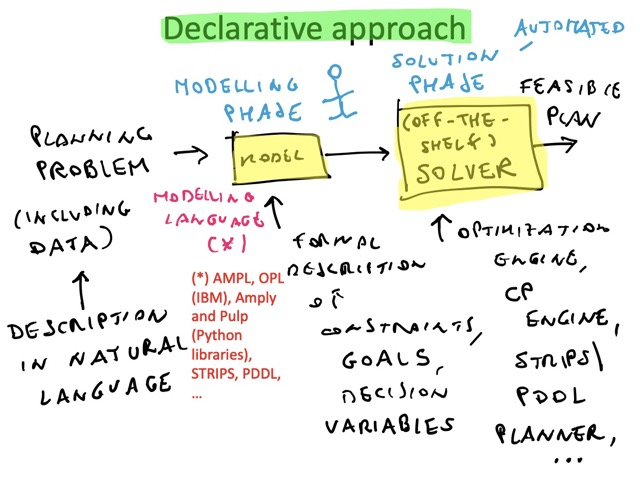
\includegraphics[scale=0.8]{descapp.jpeg}
\caption{procedura implementata} 
\label{descapp}
\end{figure}


Il che è utile dato che \hl{per agire su un problema basterà cambiare il modello} senza cambiare solver, dovrò solo cambiare il modello. È la soluzione più \hl{economico e flessibile} ma è \hl{meno performante} se in ambienti realtime devo prendere soluzioni in tempi molto stretti. Quindi in questi casi servono approcci procedurali.

Per sistemi che devono prendere soluzioni nel breve, si usa \textbf{C, C++, C#}.


% Decisioni non strutturate
\subsection{Decisioni non strutturate o destrutturate}

In questo caso \hl{non possiamo automatizzare}, quindi:

\begin{enumerate}
	\item tiro fuori i \textbf{dati aggregati}
	\item si creano statistiche con \textbf{modelli di ottimizzazione}
\end{enumerate}

Si usano degli \textbf{spreadsheet} che però non riescono a gestire big data e tendono a generare errori.

Il linguaggio più usato è \textbf{Python} ma non è la soluzione più efficiente per tutte quelle applicazioni dove il tempo di calcolo è importante.


% Decisioni semistrutturate
\subsection{Decisioni semistrutturate}

Vogliamo solo \hl{valutare le prestazione di un sistema}. Un esempio sono i sistemi che \hl{presentano un comportamento random} per motivi:

\begin{enumerate}
	\item i \textbf{server hanno un tempo di risposta} che possiamo modellare
	\item le richieste del sistema \textbf{arrivano in maniera stocastica}
\end{enumerate}

Si usano, in questo caso, \hl{metodi simulativi} tramite dei Visual Interactive Modellling System, \hl{per simulare la rete} per la quale passano le informazioni e i server ognuno con diverse proprietà di ciascun linker.



\newpage
\section{Introduzione all'ottimizzazione matematica - 30.09.22}

% Introduzione
\subsection{Introduzione}

Partiamo da un \hl{insieme di formule ed equazioni che modelleranno il problema}. Con questo modello proviamo a trovare una \hl{soluzione} al nostro problema \hl{attraverso algoritmi o risolutori}. L'output è una soluzione per il nostro modello da implementare nel mondo reale.


% Ingredienti principali
\subsection{Ingredienti principali}

Gli ingredienti principali sanno:

\begin{itemize}
	\item \textbf{dati} del problema
	\item variabili: dette anche var decisionali: scelte da fare in merito al problema. rappresentano quindi le scelte, quello su cui il decisore può intervenire
	\item vincoli: equazioni che definiscono i valori che le variabili possono assumere
	\item funzione obietivo: sarà una formula che rappresenta una misura di tipo quantitativo per capire quando è buona la soluzione che abbiamo ottenuto. quindi dovremo ottimizzare questo valore in base al contesto
\end{itemize}


Parleremo di \hl{programmazione lineare con modelli matematici} o relazioni lineari, dato che \hl{molti problemi reali si rifanno a modelli lineari}, per quanto essi possano essere complessi.


% Descrizione del problema
\subsection{Descrizione del problema}

Proviamo a risolvere un problema di mix di produzione, cioè un sistema con un impianto con 2 stabilimenti in cui:

\begin{enumerate}
	\item nel primo: diamo le materie prime e vengono realizzati i componenti in uscita
	\item nel secondo: diamo i componenti realizzati che vengono assemblati per creare il prodotto finito
	\end{enumerate}


\begin{figure}[H]
\centering
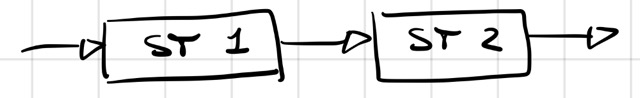
\includegraphics[scale=0.3]{st12.jpeg}
\caption{Catena tra i due stabilimenti} 
\label{st12}
\end{figure}


Supponendo di voler realizzare 2 prodotti A, B con un differente profitto. Determinare il \hl{mix di produzione}, cioè quante unità di A e B produrre la prossima settimana.
Saranno presenti dei \hl{vincoli} creati dalle risorse come i macchinari o gli addetti che potranno lavorare un numero di ore finito.


% Dati del problema
\subsection{Dati del problema}

\begin{itemize}
	\item ore di lavoro:

	\begin{table}[h!]
		\begin{center}
			\begin{tabular}{|c | c c c|} 
 				\hline
 				Stab & A & B & Addetti \\ [0.5ex]
 				\hline
	 			1 & 4 ore & 2 ore & 10 \\
 				2 & 2 ore & 4 ore & 10 \\
				\hline
			\end{tabular}
		\end{center}
		\caption{Tabella delle ore di lavoro}
		\label{taborelav}
	\end{table}

	\item ogni addetto lavora 40 ore/settimana
	
	\item profitto €/pallet:
	
	\begin{table}[h!]
		\begin{center}
			\begin{tabular}{| c c|} 
 				\hline
 				A & B \\ [0.5ex]
 				\hline
 				15k & 10k \\
				\hline
			\end{tabular}
		\end{center}
		\caption{Tabella del profitto €/pallet}
		\label{tabprof}
	\end{table}
	
	\item richiesta del prodotto nella prossima settimana:
	
	\begin{table}[h!]
		\begin{center}
			\begin{tabular}{| c c|} 
 				\hline
 				A & B \\ [0.5ex]
 				\hline
 				40 & 120 \\
				\hline
			\end{tabular}
		\end{center}
		\caption{Tabella del profitto euro/pallet}
		\label{tabprof}
	\end{table}

\end{itemize}


% Descrizione del problema con un modello matematico
\subsection{Descrizione del problema con un modello matematico}

Per \hl{effettuare una modellazione} faremo:

\begin{enumerate}
	\item \hl{identificare le variabili decisionali}:
		\begin{itemize}
			\item $x_A$: \# di pallet di prodotto A da realizzare
			\item $x_B$: \# di pallet di prodotto B da realizzare
		\end{itemize}
		
	\item \hl{definire la funzione obbiettivo (FO)}, per massimizzare il profitto

	\item \hl{definire i vincoli espressi come uguaglianza o disuguaglianza}
		\begin{itemize}
			\item vincolo 1: capacità produttiva dello stab 1 $4x_A+2x_B$ che non può superare $40*10$ cioè ore disponibili ogni settimana per un addetto * numero di addetti: $$4x_A+2x_B <= 400$$
			\item vincolo 2: capacità produttiva dello stabilimento 2 $2x_A+4x_B$ che non può superare $40*10$ cioè ore disponibili ogni settimana per un addetto * numero di addetti: $$4x_A+2x_B <= 400$$
			\item vincolo 3: vincolo sulla richiesta di A: $$x_A <= 40$$
			\item vincolo 4: vincolo sulla richiesta di B: $$x_B <= 120$$
			\item vincolo 5: vincolo di non-negatività: $$x_A, x_B >= 0$$
		\end{itemize}
		
	
\end{enumerate}

	
	
Nella forma completa il \hl{modello complessivo} è:

$$MAX=z=15x_A+10x_B$$

sottoposto ai vincoli (sv):

\begin{itemize}
	\item $4x_A+2x_B <= 400$
	\item $2x_A+4x_B <= 400$
	\item $x_A <= 40$
	\item $x_B <= 120$
	\item $x_A, x_B >= 0$
\end{itemize}


% Risolvere il modello matematico
\subsection{Risolvere il modello matematico}

\hl{Rappresentiamo sul piano cartesiano tutte le soluzioni ammissibili} cercando quella che massimizza il nostro risultato

Impostiamo delle rette per ogni vincolo:

\begin{itemize}
	\item presa $4x_A+2x_B <= 400$ poniamo = 0, a turno, $x_A$ e $x_B$: (200, 100)
	\item presa $2x_A+4x_B <= 400$ poniamo = 0, a turno, $x_A$ e $x_B$: (100, 200)
	\item presa $x_A <= 40$: (40, 0)
	\item presa $x_B <= 120$: (0, 120)
\end{itemize}


Avremo allora una \hl{regione ammissibile} dove valgono tutti i vincoli e nella quale dovrebbe essere presente la nostra soluzione ammissibile. Per trovare il punto che rende massima la funzione $z$ usiamo il \hl{metodo del gradiente}:

$$\nabla z = \left[\begin{array}{c}
	\dfrac{dz}{dx_A}\\
	\dfrac{dz}{dx_B}
\end{array}\right] = \left[\begin{array}{c}
	15\\
	10
\end{array}\right]
$$

dove $\nabla z$ sarà la massima crescita che viene rappresentata tramite (15, 10).

Tracciando una \hl{retta perpendicolare (curve di livello)} alla retta del gradiente avremo valori sempre buoni ma più bassi di quelli sul gradiente, a patto che siano validi. Troveremo in fine il punto massimo che consente di massimizzare, cioè il più estremo alla regione ammissibile sarà il nostro punto.

\hl{Seguendo la retta del gradiente troviamo che la soluzione ottimale} si trova nell'intersezione tra le rette del vincolo 2 con il 3: $x_A = 40$ $2*40+4X_B=400$ quindi $x_B=80$.

La soluzione ottimale sarà:

$$\begin{cases} 
    x_A = 40 \\ 
    2x_A+4x_B = 400
\end{cases}
\begin{cases} 
    x_A = 40 \\ 
    x_B = 80
\end{cases}$$


Si nota che lo stabilimento 2 viene saturato e quello 1 no, dal fatto che la soluzione giace sulla retta del vincolo per il quale si satura.


% Terminologia
\subsection{Terminologia}

Possiamo avere altre forme di modelli di PL:

\begin{itemize}
	\item fo da minimizzare
	\item vincoli di ugualianza
	\item vincoli $>$=
	\item variabili negative
	\item variabili non vincolate
\end{itemize}


Terminologie da sapere:

\begin{itemize}
	\item \hl{soluzione}: quella di output
	\item \hl{soluzione ammissibile}: soluzione, se esiste, che \textbf{soddisfa tutti i vincoli}
	\item \hl{soluzione inammissibile}: se \textbf{viola almeno un vincolo} 
	\item \hl{regione ammissibile}: tutti i punti che rispettano i vincoli
	\item \hl{prob inammissibile}: \textbf{regione ammissibile vuota}
	\item \hl{prob ammissibile}:
		\begin{itemize}
			\item soluzione ottima singola
			\item soluzioni multiple
			\item fo illimitata
		\end{itemize}
\end{itemize}


\begin{figure}[H]
\centering
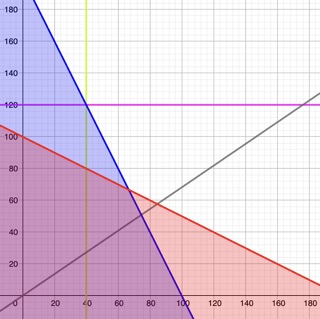
\includegraphics[scale=1]{es.jpeg}
\caption{Rappresentazione grafica esempio} 
\label{rge}
\end{figure}

	
	
% Implementazione in Python
\subsection{Implementazione in Python}

\begin{lstlisting}
import pulp as p

# 1. creazione del modello
model = p.LpProblem("ProductMix", p.LpMaximize)

# 2. definisco le variabili decisionall
x_A = p.LpVariable("x_A", cat="Continuous", lowBound=0)
x_B = p.LpVariable("x_B", cat="LpContinuous", lowBound=0)

# 3. definisco la funzione obiettivo in funzione delle variabili decisionali
model += 15 * x_A + 10 * x_B

# 4. definire i vincoli
model += 4 * x_A + 2 * x_B <= 400
model += 2 * x_A + 4 * x_B <= 400
model += x_A <= 40
model += x_B <= 120

# 5. ricolvere il problema
model.solve()

# print della soluzione
print("next week produce {} pallets of A".format(x_A.varValue))
print("next week produce {} pallets of B".format(x_B.varValue))
\end{lstlisting}


% Esercitazione
\subsection{Esercitazione}

\begin{enumerate}
	\item Massimizzare la f.o. $z = 8x_1 + 6x_2$, con i vincoli:
		\begin{itemize}
			\item $x_1 <= 5$
			\item $x_2 <= 7$
			\item $4x_1 + 3x_2 <= 29$
			\item $x_1, x_2 >= 0$
		\end{itemize}
		
		\begin{figure}[H]
		\centering
		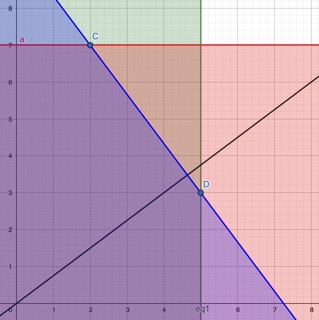
\includegraphics[scale=1]{es1.jpeg}
		\caption{Rappresentazione grafica esempio 1} 
		\label{rge1}
		\end{figure}
		
		$$\nabla z = \left[\begin{array}{c}
			\dfrac{dz}{dx_A}\\
			\dfrac{dz}{dx_B}
		\end{array}\right] = \left[\begin{array}{c}
			8\\
			6
		\end{array}\right]
		$$
		
		\hl{Abbiamo che esiste una curva di livello coincidente con lo spigolo CD, quindi abbiamo delle soluzioni ottime multiple}:
		\begin{itemize}
			\item vertice C, prendiamo allora vincolo 2 e 3:
				$$x_2 = 7 \to x_1 = 2$$
			
			\item vertice D, prendiamo allora vincolo 1 e 3:
				$$x_1 = 5 \to x_2 = 3$$
		
			\item punti del segmento CD
		\end{itemize}
		
		Quindi $z = 58$
	
	
	\item Minimizziamo la f.o. $z = 25x_1 + 22x_2$, con i vincoli:
		\begin{itemize}
			\item $x_1 + x_2 >= 5$
			\item $3x_1 + 2x_2 >= 12$
			\item $3x_1 + 6x_2 >= 18$
			\item $x_1, x_2 >= 0$
		\end{itemize}
		
		\begin{figure}[H]
		\centering
		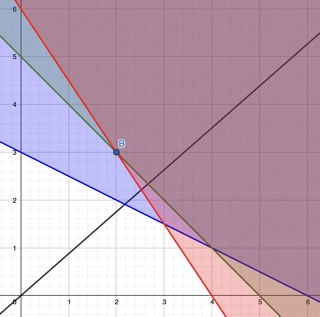
\includegraphics[scale=1]{es2.jpeg}
		\caption{Rappresentazione grafica esempio 2} 
		\label{rge2}
		\end{figure}
		
		$$\nabla z = \left[\begin{array}{c}
			\dfrac{dz}{dx_A}\\
			\dfrac{dz}{dx_B}
		\end{array}\right] = \left[\begin{array}{c}
			25\\
			22
		\end{array}\right]
		$$
		
		Per poter minimizzare, tracciando la curva di livello, trovando che la soluzione ottima si troverà dal punto B dato dall'intersezione dei vincoli 1 e 2:
		$$x_1 = 2, x_2 = 3$$
		
		Quindi $z= 116$
		
	\item Massimizziamo la f.o. $z = 2x_1 + x_2$, con i vincoli:
		\begin{itemize}
			\item $x_1 - x_2 <= 1$
			\item $2x_1 + x_2 >= 6$
			\item $x_2 >= 6$
			\item $x_1, x_2 >= 0$
		\end{itemize}
		
		\begin{figure}[H]
		\centering
		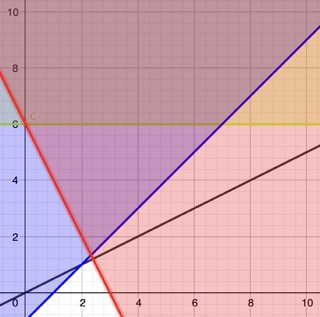
\includegraphics[scale=1]{es3.jpeg}
		\caption{Rappresentazione grafica esempio 3} 
		\label{rge3}
		\end{figure}
		
		$$\nabla z = \left[\begin{array}{c}
			\dfrac{dz}{dx_A}\\
			\dfrac{dz}{dx_B}
		\end{array}\right] = \left[\begin{array}{c}
			2\\
			1
		\end{array}\right]
		$$
		
		\hl{Non raggiungeremo la regione ammissibile, quindi il problema non ammette una soluzione ottima}.
		
	\item Minimizziamo la f.o. $z = -2x_1 + 3x_2$, con i vincoli:
		\begin{itemize}
			\item $x_1 - 2x_2 >= -2$
			\item $2x_1 - x_2 <= 3$
			\item $x_2 >= 4$
			\item $x_1, x_2 >= 0$
		\end{itemize}
		
		\begin{figure}[H]
		\centering
		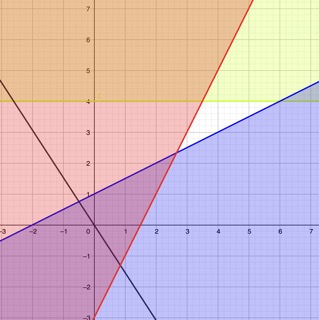
\includegraphics[scale=1]{es4.jpeg}
		\caption{Rappresentazione grafica esempio 4} 
		\label{rge4}
		\end{figure}

		
		$$\nabla z = \left[\begin{array}{c}
			\dfrac{dz}{dx_A}\\
			\dfrac{dz}{dx_B}
		\end{array}\right] = \left[\begin{array}{c}
			-2\\
			3
		\end{array}\right]
		$$
		
		\hl{La regione ammissibile e' vuota e per tanto i problema e' inammissibile, quindi non esiste un punto che soddisfa contemporaneamente tutti i vincoli}.
		
	\item L'azienda vuole decide oltre al piano di produzione anche la giusta riallocazione degli addetti (10-10) tra i due reparti.		
		Le variabili decisionali sono:
		\begin{itemize}
			\item $x_A, x_B$: i prodotti
			\item $n_p$: \# addetti allocati al reparto produzione
			\item $n_a$: \#addetti allocati al reparto assemblaggio
		\end{itemize}
		
		Quindi andremo ad aggiungere il vincolo per cui $n_p + n_a = 20$.
		
		Perciò avremo: $z = 15x_A + 10x_B$, con vincoli:
		\begin{itemize}
			\item $4x_A + 2x_B <= 40n_p$
			\item $2x_A + 4x_B <= 40n_a$
			\item $x_A <= 40$
			\item $x_B <= 120$
			\item $n_a + n_p = 20$
			\item $x_A, x_B, n_a, n_p >= 0$
		\end{itemize}
		

\end{enumerate}








\newpage
\section{Formulazioni equivalenti di un problema di programmazione lineare}


% Problema in FORMA GENERALE
\subsection{Problema in FORMA GENERALE}

In generale nella \hl{zona ammissibile} diciamo:

$$X={x \in R^n : A_x \geq b, D_x = l, x_j \geq 0}\ \ \ (*)$$
$$\forall\ \ \ j \in J \subseteq \{1,2,...,n\}$$

dove \hl{definiamo la possibilita' di vincoli di $\geq$, = e variabili $\geq$ 0}.

La funzione obiettivo è definita da: $$z = c_x\ \ \ t.c.\ \ \ z = \min z, x \in X$$

che rappresenta il \hl{problema espresso in forma generale}.


% Problema in FORMA CANONICA
\subsection{Problema in FORMA CANONICA}

Se in (*) abbiamo:

\begin{itemize}
	\item $D = 0$
	\item $J = \{1,2,...,n\}$
\end{itemize}

allora il \hl{problema si dice in forma canonica}: $$min_x\ \ \{z = c_x : A_x \geq b, x \geq 0\}$$


% Problema in FORMA STANDARD
\subsection{Problema in FORMA STANDARD}

Se in (*) abbiamo:

\begin{itemize}
	\item $A = 0$
	\item $J = {1,2,..,n}$
\end{itemize}

allora il problema è: $$min_x\ \ \{z = c_x: D_x = l, x \geq 0\}$$

Possiamo sempre \hl{ricondurci tramite trasformazioni alla forma standard}.


% Terminologia
\subsection{Terminologia}

Nella forma standard abbiamo che:

\begin{itemize}
	\item \hl{z}: la \textbf{funzione obbiettivo} per la quale trovare il valore minimo
	\item \hl{A}: \textbf{matrice dei vincoli}
	\item \hl{D}: \textbf{matrice dei coefficienti}, matrice di dimensione m x n
	\item \hl{l}: \textbf{vettore dei termini noti} vettore colonna 
	\item \hl{c}: \textbf{detto vettore dei coefficienti di costo}, vettore di riga
\end{itemize}


% Trasformazioni per ricondursi alla forma standard
\subsection{Trasformazioni per ricondursi alla forma standard}

\begin{enumerate}
	\item \hl{variabili non vincolate di segno}: $$x_j t.c. j \notin J$$

		per trasformarla possiamo \hl{sostituire a $x_j$ la somma algebrica di 2 variabili non negative}: $$x_j = x_j^+ - x_j^-$$ $$\forall\ \ \ x_j^+ \geq 0, x_j^- \geq 0$$

		Se abbiamo $k$ ($\leq n$) variabili non vincolate in segno, possiamo evitare di introdurre $k$ coppie di variabili non negative. È possibile considerare una variabile $x_0 \geq 0$ e sostituire la generica variabile non vincolata di segno con $x_j = x_j^+ - x_0$. \hl{Cosi' introduciamo "solo" $k+1$ variabili}.
	
	\item \hl{vincoli non espressi in forma di uguaglianza ($\leq$)}
		
		$$\sum_{j=i}^n a_{ij} x_j \leq b_i$$
	
		presa la \hl{variabile di Slack}: $S_i \geq 0$, avremo:
	
		$$\sum_{j=i}^n a_{ij} x_j + S_i = b_i$$
	
	
		questa variabile misura lo Slack che esiste per far si che \hl{il vincolo sia rispettato per uguaglianza} o no (vincolo $>$ 0)
		
	\item \hl{vincoli non espressi in forma di uguaglianza ($\geq$)}
	
		$$\sum_{j=i}^n a_{ij} x_j \geq b_i$$
		
		presa una \hl{variabile di Surplus}: $S_i \geq 0$, avremo:
		
		$$\sum_{j=i}^n a_{ij} x_j - S_i = b_i$$
		
	\item \hl{trasformazione di vincoli da uguaglianza in disuguaglianza} sostituendo:

		$$\sum_{j=i}^n a_{ij} x_j = b_i$$
		
		\hl{sostituendolo a}:
		
		$$\sum_{j=i}^n a_{ij} x_j \geq b_i$$
		$$\sum_{j=i}^n a_{ij} x_j \leq b_i$$
		
	\item \hl{funzione obiettivo}:
	
		Se la f.o. è $\max z = c_x$, si può trasformare:
	
		$$\max z = -\min {-z}$$

	
\end{enumerate}


% Esempio 1
\subsection{Esempio 1}

\begin{enumerate}
	\item DATI
	
		f.o.: $\min z= x_1 + 2 x_2$

		vincoli:

		\begin{itemize}
			\item $6x_1 + 4x_2 \leq 24$
			\item $4x_1 + 8x_2 \leq 32$
			\item $x_2 \geq 3$
			\item $x_1, x_2 \geq 0$
		\end{itemize}
		
	\item TRASFORMAZIONE IN FORMA STANDARd
	
		Per il primo vincolo \textbf{del tipo $\leq$, aggiungiamo una variabile non negativa} (slack):

		$$6x_1 + 4x_2 + x_3 = 24$$

		per il secondo vincolo operiamo in maniera analoga :

		$$4x_1 + 8x_2 + x_4 = 32$$

		per il terzo vincolo \textbf{del tipo $\geq$, aggiungiamo una variabile ausiliaria negativa}:
		
		$$x_2 - x_5 = 3$$

		vincolo sulle variabili:

		$$x_1, x_2, x_3, x_4, x_5 \geq 0$$

		quindi nella formulazione standard avremo $j = 1,2,3,4,5$ quando in precedenza avevamo: $j = 1, 2$
	
\end{enumerate}


% Esempio 2
\subsection{Esempio 2}

\begin{enumerate}
	\item DATI
	
		f.o.: $\max z = z_1 + z_2$

		vincoli:

		\begin{itemize}
			\item $8x_1 + 6x_2 \geq 48$
			\item $5x_1 + 10x_2 \geq 50$
			\item $13x_1 + 10x_2 \leq 130$
			\item $x_1 \geq 0$
		\end{itemize}
		
	\item TRASFORMAZIONE IN FORMA STANDARD
	
		Dato che non abbiamo vincoli su $x_2$ poniamo:
		
		$$x_2 = x_2^+ - x_2^-$$
		
		la f.o. sarà:
		
		$$\max z = -\min -z = -x_1 -x_2 = -x_1 -x_2^+ + x_2^-$$
		
		invece i vincoli:
		
		\begin{itemize}
			\item $8x_1 + 6x_2^+ - 6x_2^- - x_3 = 48$
			\item $5x_1 + 10_2^+ - 10x_2^- - x_4 = 50$
			\item $13x_1 + 10_2^+ - 10x_2^- + x_5 = 130$
			\item $x_1, _2^+, x_2^-, x_3, x_4, x_5 \geq 0$
		\end{itemize}
	
\end{enumerate}


\newpage
\section{Optimization models review}

% Scheduling
\subsection{Scheduling}

Nell'ambito dei problemi dello scheduling abbiamo degli elementi ben specificati:

\begin{itemize}
	\item \hl{task/job} già assegnati
	\item $n$ \hl{macchine/processori}
	\item potremmo attrezzare le macchine con dei \hl{tools}
\end{itemize}

Intendiamo \hl{allocare i tasks alla macchine in "overtime"} quindi capire anche la \hl{fascia temporale nella quale eseguire il task}. Potrebbe esserci un unico tempo di esecuzione oppure un task può avere dei tempi di esecuzione differenti su macchine differenti. 

L'output sarà un diagramma di Ganth.

\hl{I task possono avere degli istanti di rilascio} dove non potrebbe essere rilasciato dopo un certo istante di tempo (\hl{ready time}).

Possono esserci delle \hl{relazioni di precedenza tra i tasks}. Quindi non posso effettuare un task se prima non ho concluso l'altro.

Il diagramma mi dice nel tempo a che macchina è associato quale task ed in quali intervalli di tempo e con quale tool.


% Project scheduling
\subsection{Project scheduling}

Per progetto intendiamo un \hl{insieme di tasks che sono realizzati al fine di raggiungere un goal}. La caratteristica di un progetto è che nel complesso le attività non sono mai state eseguite in precedenza.

Le \hl{caratteristiche di un progetto} sono:


\begin{itemize}
	\item \textbf{durata delle attività} che nota
	\item ha \textbf{a capo un Project Manager}: responsabile del progetto e dei tempi di realizzazione, costi di produzione, ecc...
\end{itemize}

Un progetto è \hl{rappresentato da diverse attivita'} in una tabella fornita dal Project Manager:


\begin{table}[h!]
	\begin{center}
	\begin{tabular}{|c | c c |} 
		\hline
		Attività & Durata stimata $d_i$ & Predecessori \\ [0.5ex]
		\hline
 		1 & 10 & - \\
		2 & 10 & - \\
		3 & 10 & 1 \\
		4 & 10 & 1, 2 \\
		\hline
		\end{tabular}
	\end{center}
	\caption{Tabella di ore di lavoro e predecessioni delle attività}
	\label{tabatt}
\end{table}


e in un diagramma aciclico (Activity On Node (AoN)):


\begin{figure}[H]
\centering
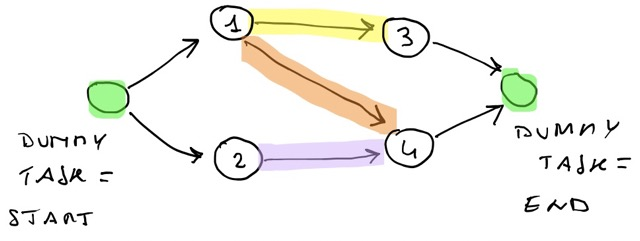
\includegraphics[scale=0.4]{aon.jpeg}
\caption{Diagramma Activity On Node} 
\label{aon}
\end{figure}


dove abbiamo degli "archi" che rappresentano le predecessioni. Avremo anche dei \hl{vertici fittizzi}:

\begin{itemize}
	\item start: lo colleghiamo tutte le attività che non hanno predecessori
	\item end: ci colleghiamo tutte le attività finali
\end{itemize}

Una funzione fondamentale del Project Manager è la possibilità di accelerare alcune attività agendo su:

\begin{itemize}
	\item \hl{Variabili decisionali}:
		
		nel nostro caso, è lo \hl{start time $s_i$}. Ipotizziamo che il progetto inizi al tempo $t = 0$, quindi per ogni task abbiamo che:

			$$s_i \geq 0\ \ \ \forall\ \ \ i \in TASKS$$

		In più possiamo definire \hl{$T \geq 0$ tempo di completamento del progetto} (\textbf{completion time}).

		Minimizziamo il completion time:

			$$\min z = T$$

		con $z = 1T + 0s_1 + 0s_2 + ... + 0s_n$
		
		
	\item \hl{relazioni di precedenza}:
	
		relazioni che portano alcuni nodi a dipendere da altri:
		
		$$
		p_{ij}=
		\begin{cases} 
		    1 \Leftrightarrow i \in j \\ 
		    0 altrimenti
		\end{cases}$$
		
		con \hl{$p_{ij}$ matrice} costate e binaria:
		
		$$p =
		\left[ {\begin{array}{cccc}
		    0 & 0 & 1 & 1 \\
			0 & 0 & 0 & 1 \\
		    0 & 0 & 0 & 0 \\
		    0 & 0 & 0 & 0 \\
		\end{array} } \right]$$
		
	
	\item \hl{vincoli di precedenza}:
	
		Sia \hl{$T$ maggiorante del tempo di completamento delle task}:
			$$s_i + d_i \leq T$$

		allora:

			$$p_{ij} (s_i + d_i) \leq s_j\ \ \ \forall\ \ \ i,j \in TASKS$$

		Possiamo avere che:

		\begin{itemize}
			\item \hl{$p_{ij} = 1$}: allora \textbf{$i$ è predecessore di $j$} quindi il tempo di inizio del task $j$ deve essere successivo o uguale al task $i$ cioè $s_i + d_i$
	
			\item \hl{$p_ij = 0$}: $i$ non è predecessore quindi avremo $0 \leq s_j$ allora il vincolo è ridondante
		\end{itemize}
		
		scriviamo allora:
 
		$$s_i + d_i \leq s_j\ \ \ \forall\ \ \ i,j \in TASKS,\ p_{ij} \geq 0$$


\end{itemize}


% Esempio
\subsection{Esempio }

Un modello espanso per problemi di istanza:

\begin{enumerate}
	\item funzione obiettivo: $\min z = T$
	\item vincoli:
		\begin{itemize}
			\item $s_1 + 10 \leq T$
			\item $s_2 + 10 \leq T$
			\item $s_3 + 10 \leq T$
			\item $s_4 + 10 \leq T$
			\item $s_1 + 10 \leq s_3 (p_{13} = 1)$
			\item $s_1 + 10 \leq s_4 (p_{14} = 1)$
			\item $s_2 + 10 \leq s_4 (p_{24} = 1)$
			\item $s_1, s_2, s_3, s_4 \geq 0$
			\item $T \geq 0$
		\end{itemize}
\end{enumerate}


% Velocizzazione del progetto
\subsection{Velocizzazione del progetto}

Il Project Manager ha un \hl{budget} per poter velocizzare il progetto.

Se considero un \hl{task $i$ con durata non costante ($d_i^N$)}, avremo un valore nominale che dipende da un budget extra.

Il più semplice è l'\hl{andamento lineare} dove all'aumentare delle risorse la durata si riduce in modo lineare. Il che è vero finché non si incontra un \hl{vincolo inferiore $d_i^m$}.


Le \hl{3 risorse} alle quali si possono far riferimento sono le \hl{3M}:

\begin{itemize}
	\item Man
	\item Machine
	\item Money
\end{itemize}


quindi $d_i = d_i^N$.


\begin{figure}[H]
\centering
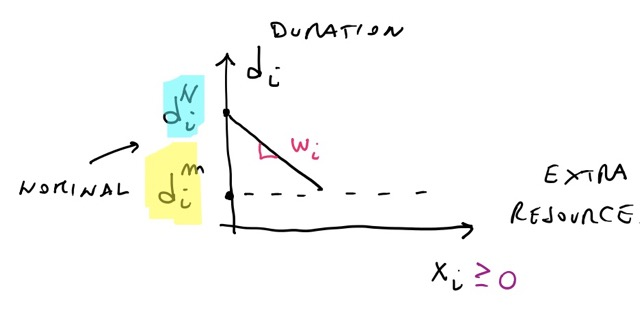
\includegraphics[scale=0.4]{budget.jpeg}
\caption{Diagramma budget} 
\label{budget}
\end{figure}


con:

\begin{itemize}
	\item \hl{pendenza w}: \textbf{riduzione della durata del task $i$} per unità di extra risorse (mesi di lavoro / k euro)
	\item $d_i = d_i^N - w_i x_i \geq d_i^m$ vincolo del valore minimo per task
	\item $x_i$: denaro usato per il task $i$
	\item $B$: budget totale

\end{itemize}


% Esempio velocizzazione progetto
\subsection{Esempio velocizzazione progetto}

Avremo un modello con:

\begin{enumerate}
	\item funzione obiettivo: $\min z = T$
	\item vincoli:
		
		\begin{itemize}
			\item $s_i + d_i^N - w_i x_i \leq T\ \ \ \forall\ \ \ i \in TASKS$
			\item $s_i + d_i^N - w_i x_i \leq s_j\ \ \ \forall\ \ \ i, j \in TASKS, p_{ij} = 1$
			\item $d_i^N - w_i x_i \geq d_i^m\ \ \ \forall\ \ \ i \in TASKS$
			\item $\sum_{i \in TASKS} x_i \leq B$
			\item $T \geq 0$
			\item $s_i \geq 0\ \ \ \forall\ \ \ i \in TASKS$
			\item $x_i \geq 0\ \ \ \forall\ \ \ i \in TASKS$
		\end{itemize}
\end{enumerate}


% Low sizing models
\subsection{Low sizing models}

Sono in genere usati da aziende manifatturiere. 


\begin{figure}[H]
\centering
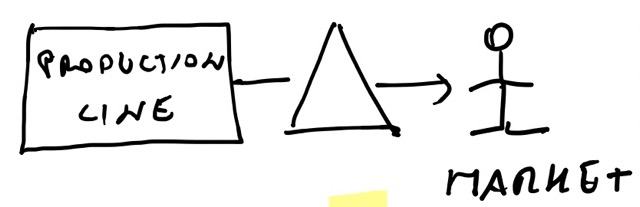
\includegraphics[scale=0.3]{prodline.jpeg}
\caption{Processo produtivo} 
\label{procprod}
\end{figure}


Supponendo di avere un \hl{tasso di domanda $d$} costante in base al tipo di prodotto. Ogni tipo di prodotto si differenzia dagli altri con una piccola modifica come può essere un differente gusto per una produzione di yogurt.

Questa differenziazione porta ad un \hl{costo di setup} delle macchine che andranno pulite, generando un costo fisso $k$.

Il livello di scorte sarà rappresentato con dei picchi con ampiezza $q$:


\begin{figure}[H]
\centering
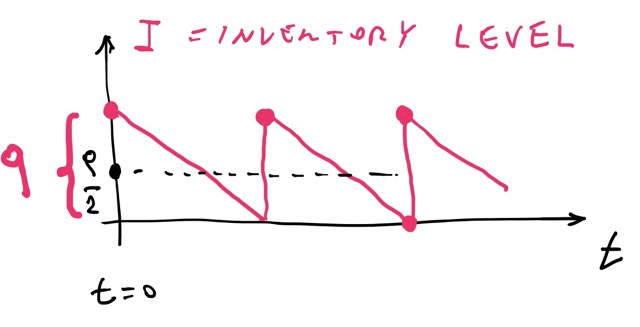
\includegraphics[scale=0.3]{invlev.jpeg}
\caption{Livello di inventario} 
\label{invlev}
\end{figure}


avendo una domanda costante, avremo una diminuzione lineare nello scorte di magazzino.

Ovviamente avremo dei \hl{costi medi di stockaggio $h$} dato che le scorte si "muoveranno" scambiandosi con altre scorte che entrano nel magazzino. Quindi andremo a calcolare il costo in base alla giacenza del \hl{numero di scorte medie $\frac{q}{2}$}.

In base alla strategia avremo:

\begin{enumerate}
	\item \hl{caso estermo}:
	
		gestione di tipo \textbf{just in time} dove \textbf{produco solo sotto commissione del cliente}.

		Avremo quindi:
		
		\begin{itemize}
			\item \textbf{livello di scorte molto basso} con un livello medio delle scorte molto basso e dei \textbf{costi di stockaggio bassi}
			\item \textbf{maggioramento dei costi del setup}
			\item pago $k$ più volte durante l'anno
		\end{itemize}
		
	\item \hl{caso produzione annua}:
	
		si produce un \textbf{quantitativo pari alla domanda annua}.
		
		Avremo quindi:
		
		\begin{itemize}
			\item grandi \textbf{costi di stockaggio}
			\item pago $k$ solo una volta all'anno
		\end{itemize}

\end{enumerate}


\begin{figure}[H]
\centering
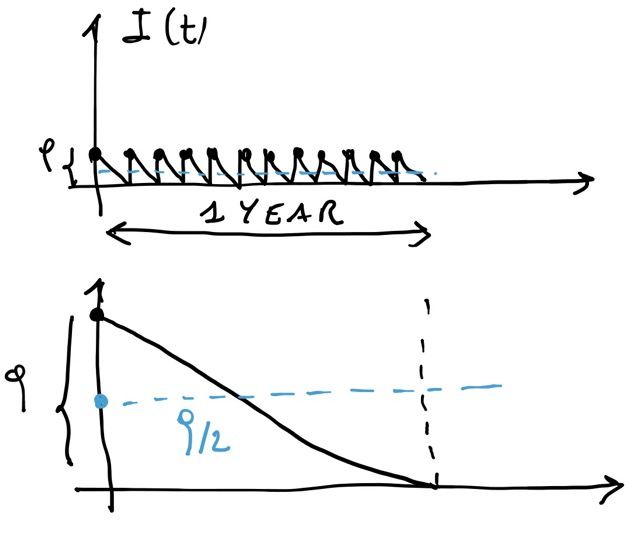
\includegraphics[scale=0.3]{casipart.jpeg}
\caption{Casi particolari} 
\label{casipart}
\end{figure}


% Scrivere il modello di ottimizzazione
\subsection{Scrivere il modello di ottimizzazione}

Le fasi da seguire prevedono la scrittura di:

\begin{enumerate}
	\item \hl{variabili decisionali}: variabile matematica per descrivere la mia decisione
	\item \hl{funzione obiettivo}: costo totale annuale composto dal \textbf{costo di scorta e quello di setup}
\end{enumerate}

Avremo allora:

$$z = k \frac{d}{q} + h \frac{q}{2} $$


Per la \hl{soluzione ottima}, faccio il gradiente:

$$\frac{dz}{dq} = 0 \Leftrightarrow -k \frac{d}{q^2} + \frac{h}{2} = 0$$


Concludiamo che il \hl{lotto economico}, per minimizzare i costi, sarà raggiunto da:

$$q^* = \sqrt{\frac{2kd}{h}}$$


\begin{figure}[H]
\centering
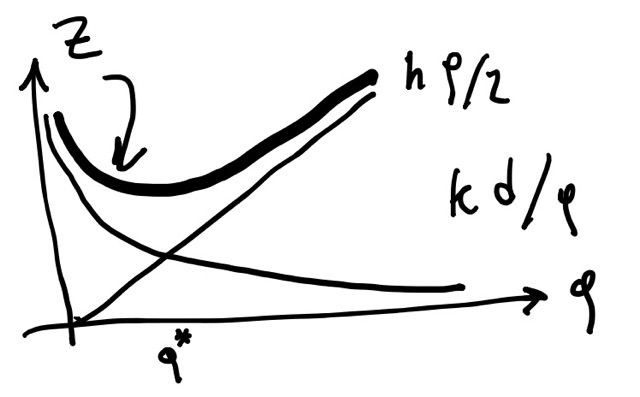
\includegraphics[scale=0.3]{lottoec.jpeg}
\caption{Caso di lotto economico} 
\label{lottoec}
\end{figure}



Questo modello \hl{nella pratica ha dei limiti} dati i possibili vincoli come:

\begin{itemize}
	\item spazio limite di un magazzino
	\item produzione di più prodotti contemporaneamente
	\item vincolo di immobilizio
	\item vincolo sul capitale
	\item ecc ...
\end{itemize}


Associati al vincolo di immobilizzo possiamo avere anche un \hl{limite nei prodotti che posso fare di A e di B}. Se si ipotizza una domanda costante, ho che il \hl{costo totale annuale $z$} sarà data dal costo annuale di A e di B:

$$z = (k_A \frac{d_A}{q_A} + h_A \frac{q_A}{2}) + (k_B \frac{d_B}{q_B} + h_B \frac{q_B}{2})$$


Avremo che $z$ è dato da 2 termini uno che dipende da A ed uno da B. Per noi supponiamo che $k_A = k_B = k$.

Di conseguenza anche i lotti di approvvigionamento possono essere diversi. Quindi, quando è necessario, avremo che dovremo \hl{decidere quante confezioni produrre di A e quante di B}.

Nel \hl{caso peggiore ipotizzo che la produzione contemporanea di 2 lotti}, quindi non dovrà superare la capacità di magazzino $Q$:

$$q_A + q_B \leq Q\ \ \ \forall\ \ \ q_A, q_B \geq 0$$

dove la produzione contemporanea indica la \hl{sovrapposizione dei denti di sega}.

Se la \hl{capacita' del magazzino e' minore del lotto economico, la soluzione ottima sara' la nostra capacita'} e non più $q^*$.

Per il \hl{vincolo del capitale}, indiciamo con $c_A$ e $c_B$ il valore di un singolo prodotto di A e B allora:

$$c_Aq_A + c_Bq_B \leq C$$

con $C$ capitale massimo.

Dal \hl{punto di vista grafico} avremo 2 variabili $q_A$ e $q_B$ con dei vincoli sono di tipo lineare:

$q_A + q_B \leq Q$
$c_Aq_A + c_Bq_B \leq C$


\begin{figure}[H]
\centering
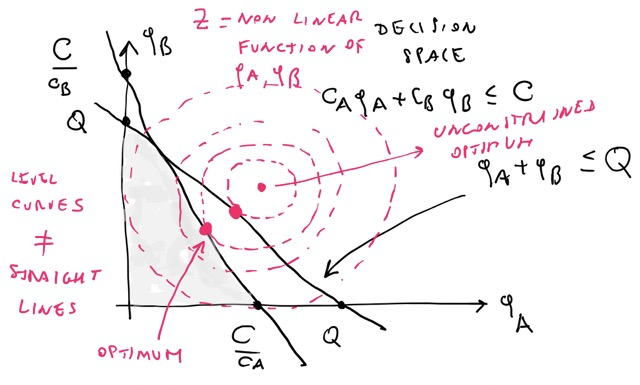
\includegraphics[scale=0.4]{linlivnonlin.jpeg}
\caption{Grafico con linee di livello non lineari} 
\label{linlivnonlin}
\end{figure}


La \hl{funzione obiettivo non e' lineare} dato che $q_A$ e $q_B$ sono al denominatore. Le \hl{curve di livello non sono delle rette} ma saranno concentriche (su ognuna il costo è sempre costante).

Avremo una \hl{soluzione ottima dalla curva di livello tangente all'insieme di ammissibilita'}. Si vado allora a prendere le curve peggiori fino ad arrivare a quella che interseca la regione ottima.


% Algoritmo del simplesso
\subsection{Algoritmo del simplesso}

Ogni problema di ottimizzazione lineare si può \hl{trasformare in forma standard}. Prendiamo un f.o.:

$$\min z = \underline{c}^T \underline{x}$$

e dei vincoli:

\begin{itemize}
	\item $\underline{\underline{A}}\ \underline{x} = \underline{b}$
	\item $\underline{x} \geq 0$
	\item $n > m$
\end{itemize}

con $n$ righe e $m$ colonne delle matrice $\underline{\underline{A}}$.

Utilizziamo l'\hl{operazione di Pivot}, quindi il vincolo:

$$\underline{\underline{A}}\ \underline{x} = \underline{b}$$

sarà:


$$
\left[ {\begin{array}{cccc}
	4 & 1 & 5 & 7 \\
	2 & 3 & 2 & 1 \\
\end{array} } \right]
\left[ {\begin{array}{c}
	x_1 \\
	x_2 \\
	x_3 \\
	x_4 \\
\end{array} } \right]
=
\left[ {\begin{array}{c}
	10 \\
	10 \\
\end{array} } \right]
$$

Il Pivot che ci viene assegnato è:

$$(r, s) = (1, 3)$$

alla quale coordinata corrisponde il valore della prima riga e terza colonna: $5$.

Dai dati \hl{creiamo un sistema di eq lineari}:

$$
\begin{cases} 
    4x_1 + x_2 + 5x_3 + 7x_4 = 10 \\ 
    2x_1 + 3x_2 + 2x_3 + 1x_4 = 10 
\end{cases}
$$

Per eseguire l'operazione di Pivot andremo a far si che \hl{in corrispondenza della colonna di Pivot ($s$) ci sia solo un vettore unitario}:

$$
\left[ {\begin{array}{cccc}
	? & ? & 1 & ? \\
	? & ? & 0 & ? \\
\end{array} } \right]
\left[ {\begin{array}{c}
	x_1 \\
	x_2 \\
	x_3 \\
	x_4 \\
\end{array} } \right]
=
\left[ {\begin{array}{c}
	? \\
	? \\
\end{array} } \right]
$$

Gli steps da seguire sono:

\begin{enumerate}
	\item facciamo \hl{$\frac{r}{a_{rs}}$}, con:
		
		\begin{itemize}
			\item $r$: riga Pivot
			\item $a_{rs} \neq 0$: valore che si trova dal Pivot, nel nostro caso $5$
		\end{itemize}
		
		Diremo quindi che:
		
		$$a_{rj} = \frac{a_{rj}}{a{rs}}\ \ \ \forall\ \ \ j = 1, ..., n+1$$

		$$
		\left[ {\begin{array}{cccc}
			\frac{4}{5} & \frac{1}{4} & 1 & \frac{7}{5} \\
			? & ? & 0 & ? \\
		\end{array} } \right]
		\left[ {\begin{array}{c}
			x_1 \\
			x_2 \\
			x_3 \\
			x_4 \\
		\end{array} } \right]
		=
		\left[ {\begin{array}{c}
			2 \\
			? \\
		\end{array} } \right]
		$$
	
	\item per ogni riga non Pivot $i \neq r$ applichiamo il principio di equivalenza per eq non lineari:
	
		$$\text{riga } i = \text{riga } i + (-a_{is}) * \text{nuova riga } r$$
		
		in questo caso andiamo a sommare $-2$ in modo da avere la configurazione $(1, 3) = 1$ e $(2, 3) = 0$.
		
		Diremo quindi che:
		
		$$a_{ij} = a{ij} + (-a{is})a_{rj}\ \ \ \forall\ \ \ i = 1, ..., m;\ i \neq r$$
		
		\begin{table}[!h]
		    \begin{center}
				\def\arraystretch{2}
		    	\begin{tabular}{| c c c c | c |}
		    	    \hline
		    	    \textbf{col 1} & \textbf{col 2} & \textbf{col 3} & \textbf{col 4} & \textbf{ris} \\\hline
		    	    $\ \ 2$ & $\ \ 3$ & $\ \ 2$ & $\ \ 1$ & $\ 10\ +$ \\
		     		$-\frac{8}{5}$ & $-\frac{2}{5}$ & $-2$ & $-\frac{14}{5}$ & $-4\ =$ \\\hline
		     		$\ \frac{2}{5}$ & $\ \frac{13}{5}$ & $\ \ 0$ & $-\frac{9}{5}$ & $\ \ 6$ \\
					\hline
		    \end{tabular}
		\end{center}
		\end{table}
		
		quindi abbiamo:
		
		$$
		\left[ {\begin{array}{cccc}
			\frac{4}{5} & \frac{1}{4} & 1 & \frac{7}{5} \\
			\frac{2}{5} & \frac{13}{5} & 0 & -\frac{9}{5} \\
		\end{array} } \right]
		\left[ {\begin{array}{c}
			x_1 \\
			x_2 \\
			x_3 \\
			x_4 \\
		\end{array} } \right]
		=
		\left[ {\begin{array}{c}
			2 \\
			6 \\
		\end{array} } \right]
		$$
	
\end{enumerate}


% Tableau
\subsection{Tableau}

Possiamo quindi riscrivere la forma standard con il Tableau con una \hl{forma tabellare} del tipo:

$$ \underline{\underline{\overline{A}}} =
\left[ {\begin{array}{cc}
	\underline{\underline{A}} & \underline{b} \\
	c^T & 0 \\
\end{array} } \right]
$$

dove $m$ righe e $n$ colonne.

I nostri problemi hanno variabili continue dove usando l'algoritmo del simplesso avremo come \hl{forma generale}:

$$\min c_1x_1 + ... + c_n x_n$$

per i vincoli invece:

\begin{itemize}
	\item $a_{11}x_1 + ... + a_{an}x_n = b_1$
	\item \dots
	\item $a_{m1}x_1 + ... + a_{mn}x_n = b_m$
	\item $x_1, ..., x_n \geq 0$
\end{itemize}

\hl{Assumiamo che}:

\begin{enumerate}
	\item $n > m$
	\item $\text{rank}(\underline{A}) = n$
\end{enumerate}

così \hl{non avremo vincoli ridondanti}.

Applichiamo poi la definizione di \hl{insieme di base $B$} (con $\underline{x}_B \in R^m$) ed \hl{insieme non di base $N$} (con $\underline{x}_N \in R^{n-m}$).

quindi avrò che:

$$\underline{x} = (\underline{x}_B, \underline{x}_N)$$

allora:

$$\underline{\underline{A}} = [\underline{\underline{B}} | \underline{\underline{N}}]$$

Se la matrice \hl{$B$ non e' singolare posso ricavare una soluzione} imponendo $$\underline{x}_N:=0$$

Per le \hl{variabili $B$} avremo:

$$\underline{\underline{B}}\ \underline{x}_B = \underline{b}\ \ \ \to\ \ \ \underline{x}_B = \underline{\underline{B}}^{-1}\ \underline{b}$$

sarà anche \hl{ammissibile se $\geq 0$}

Tutto questo grazie al \hl{teorema fondamentale} che dice:

\begin{enumerate}
	\item se un problema ha \textbf{soluzione ammissibile}, allora almeno una \textbf{è di base}.
	\item se \textbf{ammette soluzioni ottime}, c'è n'è almeno \textbf{una di base}
\end{enumerate}


Le soluzioni di base sono quindi più comode dato che sono più piccole in un insieme $R^n$ di soluzioni non ammissibili, ammissibili e ottime.


\begin{figure}[H]
\centering
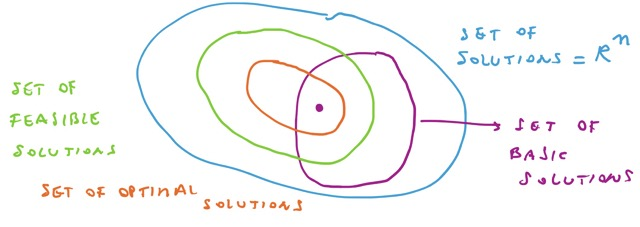
\includegraphics[scale=0.4]{inssol.jpeg}
\caption{Insiemi delle soluzioni} 
\label{inssol}
\end{figure}


Capiamo allora che i \hl{modi per poter scegliere $x_B$} saranno dati dal numero di combinazioni di $n$ elementi di classe $m$:

$$ \binom{n}{m} = \frac{n!}{m!(n-m)!}$$


% Esempio Tableau
\subsection{Esempio Tableau}

Funzione obiettivo:

$$\min z = 2x_1 + 3x_2 + 4x_3 - 5x_4$$

vincoli:

\begin{itemize}
	\item $x_1 - x_2 + x_3 + 2x_4 = 3$
	\item $2x_2 + x_4 = 7$
	\item $x_1 + 2x_3 = 10$
	\item $x_1, x_2, x_3, x_4 \geq 0$
\end{itemize}

Supponiamo: $m = 3$ e $n = 4$.

e scegliamo sull'insieme di tutte le variabili, combinazioni lineari di tanti numeri quante sono le equazioni. Prendiamo per esempio:

\begin{itemize}
	\item $\underline{x}_B = (x_1, x_3, x_4)$
	\item $\underline{x}_N = (x_2)$
\end{itemize}

Andiamo allora a prendere i termini delle variabili e a inserirli in $A$:

$$A =
\left[ {\begin{array}{cccc}
	1 & -1 & 1 & 2\\
	0 & 2 & 0 & 1\\
	1 & 0 & 2 & 0\\
\end{array} } \right]
$$

Dalla f.o. troviamo:

$$c^T = (2, 3, 4, -5)$$

Andremo poi a distribuire a ogni matrice i suoi dati:

$$B =
\left[ {\begin{array}{ccc}
	1 & 1 & 2 \\
	0 & 0 & 1 \\
	1 & 2 & 0 \\
\end{array} } \right]
$$

$$\underline{c}_B = (2, 4, -5)$$

$$N =
\left[ {\begin{array}{c}
	-1 \\
	2 \\
	0 \\
\end{array} } \right]
$$

nel nostro caso c sarà:

$$\underline{c}_N = (3)$$


possiamo allora riscrivere come:

$\min \underline{c}^T_B \underline{x}_B + \underline{c}^T_N \underline{x}_N$


% Forma canonica
\subsection{Forma canonica}

Con le operazioni Pivot \hl{poniamo il problema in forma canonica rispetto a una base}:


$$
\left[ {\begin{array}{ccccc}
	2  & 1  & 4   & -2 & 10\\
	1  & 2  & 4   & 2  & 10\\
	10 & 10 & -2  & 2  & 0 \\
\end{array} } \right]
$$


dove:

\begin{itemize}
	\item \textbf{vincoli} (prime righe):

		\begin{itemize}
			\item[] $2x_1 + x_2 + 4x_3 - 2x_4 = 10$
			\item[] $x_1 + 2x_2 + 4x_3 - 2x_4 = 10$
		\end{itemize}

	\item \textbf{funzione obiettivo} (ultima riga): $$10x_1 + 10x_2 - 2x_3 + 2x_4 + (-z) = 0$$

\end{itemize}

quindi la \hl{funzione obiettivo} è:

$$\min z = 10x_1 + 10x_2 - 2x_3 + 2x_4 + 0$$

e avrà ovviamente tutte le variabili $\geq  0$.


Se effettuo un'\hl{operazione di Pivot} su $(0, 3)$:


$$
\left[ {\begin{array}{ccccc}
	-1 & -0.5 & -2 & 1 & -5\\
	3  &   3  & 8  & 0 & 20\\
	12 &   11 & 2  & 0 & 10\\
\end{array} } \right]
$$

ed un'altra operazione di Pivot su $(1, 1)$:


$$
\left[ {\begin{array}{ccccc}
	-0.5 & 0 & -0.6   & 1 & -1.6\\
	1  	 & 1 & 2.6    & 0 &  6.6\\
	1    & 0 & -27.6  & 0 & -63.3\\
\end{array} } \right]
$$


Il \hl{sistema vincolare e' risolto per $x_2$ e $x_4$} dato che sono quelle \hl{scelte dal Pivot}. Poniamo poi $x_1, x_3 := 0$ ed avremo:

$$x_4 = -1.6,\ x_2 = 6.6$$

quindi avremo una \hl{soluzione base}:

$$\underline{x} = (0, 6.6, 0, -1.6)$$

Questa soluzione è \hl{inammissibile perche' $x_4 \leq 0$} quindi non è Basic Feasible Solution (BFS).

Per esprimere la forma canonica diciamo che gli \hl{indici di colonna delle variabili di $B$ e $N$} sono:

$$I_B = <1, 3>$$
$$I_N= <0, 2>$$

possiamo dire la \hl{posizione delle variabili in base alle equazioni} con:

$$\beta(0) = 3$$
$$\beta(1) = 1$$

\hl{Una forma canonica mi da una soluzione base} andando a porre le \hl{variabili non di base $= 0$} e trovando quelle di base.

Il \hl{valore in basso a destra del Tableau} rappresenta il valore:

$$z = x_1 -27.3x_3 + 63.3$$

dove essendo $x_1$ e $x_3$ non di base:

$$\overline{z} = 63.3$$

quindi rappresenta il \hl{valore della soluzione di base associato a questa forma canonica}.


% Generalizzazione forma canonica
\subsection{Generalizzazione forma canonica}

Generalizzando avrò come \hl{funzione obiettivo}:

$$\min z = \sum_{j \in  I_N} \overline{c}_jx_j + \overline{z}$$

e con \hl{vincoli}:

$$x_{\beta(i)} + \sum_{j \in  I_N} \overline{a}_{ij}x_j = \overline{b}_i\ \ \ \forall\ \ \ i = 0, ..., m - 1$$

con ovviamente $x_j \geq 0, j \in J_N \cup J_B$

L'\hl{equazione di base associata} sarà:

$$x_j := 0\ \ \ \forall\ \ \ j \in J_N$$
$$x_{\beta(i)} = \overline{b}_i \leq \geq 0\ \ \ \forall\ \ \ i = 0, ..., m-1$$

\hl{Pseudocodice} dell'algoritmo del simplesso:

Andremo a:

\begin{enumerate}
	\item trovo la prima \hl{BFS}
	\item in loop faccio:
		\begin{itemize}
			\item un \hl{test di ottimalita'}
			\item se fallisce allora \textbf{sarà migliorabile}
			\item allora mi \textbf{muovo nei dintorni} del suo spazio per migliorare la situazione
		\end{itemize}
	\item se trovo una soluzione di base ammissibile ottima faccio un \hl{analisi per capire se e' unica} o meno
\end{enumerate}


Avremo la \hl{forma generale} quando è \hl{$\leq$ e $\underline{b} \geq 0$}.

Per il \hl{test di ottimalita' in forma canonica}:

$$\min z = \sum_{j \in  I_N} \overline{c}_jx_j + \overline{z}$$

il che significa che per $\underline{x}$ la soluzione ammissibile sarà:

$$z(\underline{x}) = \sum_{j \in  I_N} \overline{c}_jx_j + \overline{z}$$

allora \hl{se $\overline{c}_j \geq 0$ avremo una forma ottimale}, dato che $z(\underline{x}) \geq \overline{z}$

Se \hl{parto dalla soluzione di base ammissibile e prendo una variabile fuori base rendendola positiva}, la funzione obiettivo varia in base alla relazione:

$$z = \sum_{j \in J_N} \overline{c}_j...(slide)$$

cioè \hl{$x_j = 0 \to 1$}

Avremo quindi che la variazione della funzione obiettivo è uguale al coefficiente di posto ridotto $\overline{c}_j$: \hl{$\Delta z = \overline{c}_j$}.

Riusciamo così a \hl{diminuire $z$} il che ci piace perché stiamo minimizzando.

Se il \hl{test di ottimalita' fallisce} perché esiste una variabile di base con coefficiente di costo ridotto negativo potremo avere 2 situazioni:


\begin{figure}[H]
\centering
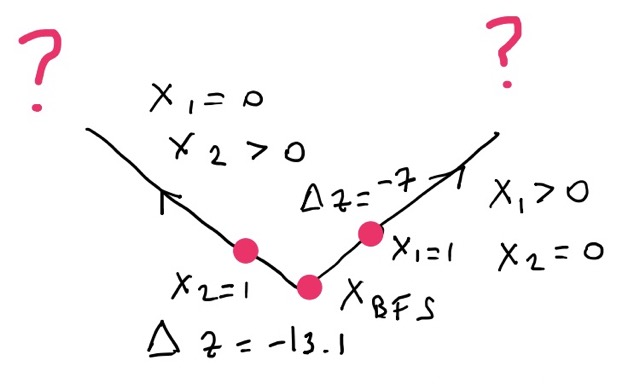
\includegraphics[scale=0.2]{2sol.jpeg}
\caption{Soluzioni per ottimalità} 
\label{2sol}
\end{figure}


Se ho più variabili di base negative allora devo capire \hl{quale delle due devo perturbare}, cioè rendere $> 0$, e la \hl{scegliamo con un "euristica"} che è una scelta algoritmica basata sull'intuizione e info pregresse.

Sceglieremo come variabile, detta variabile entrante, quella con \hl{coefficiente di costo piu' negativo}:

$$x_s = \min_{j \in I_N} \overline{c}_j$$

quindi se $\Delta z = \overline{c}_s x_s$

Se dobbiamo \hl{minimizzare avremo l'interesse e far raggiungere a $x_s$ il valore piu' elevato possibile} dato che ci sarà un miglioramento.

Applichiamo un \hl{vincolo sul massimo valore che $x_s$ puo' raggiungere}:

$$x_s = 0 \to\ > 0$$
$$x_j = 0\ \ \ \forall\ \ \ j \in I_N,\ j \neq s$$

allora avremo:
$$\min z = \overline{c}_s x_s + \overline{z}$$

con vincoli:

\begin{itemize}
	\item $x_{\beta(i)} + \overline{a}_{is}x_s = \overline{b}_i\ \ \ \forall\ \ \ i = 1, ..., m$
	\item $x_j \geq 0\ \ \ \forall\ \ \ j = 1, ..., m$
\end{itemize}

avremo quindi che \hl{$x_s$ cresce fino al non superamento dei vincoli}:

$$x_{\beta(i)} = \overline{b}_i - \overline{a}_{is}x_s \geq 0$$

A questo punto avremo 2 casi possibili:
\begin{enumerate}
	\item avremo:
		$$\overline{a}_{is} \leq 0\ \ \ \forall\ \ \ i = 1, ..., m$$
		allora:
		$$x_{\beta(i)} \geq 0\ \ \ \forall\ \ \ x_s \to +\infty$$
		
		con: $z \to -\infty$
	
	\item avremo:
		$$\exists\ i : \overline{a}_{is} > 0$$

		per calcolare il \hl{massimo valore che $x_s$ puo' assumere} è dato da:

		$$-\overline{a}_{is} x_s \geq -\overline{b}_i$$
		$$\Rightarrow x_s \leq \frac{\overline{b}_i}{\overline{a}_{is}}\ \ \ \forall\ \ \ i = 1, ..., m;\ \overline{a}_{is} > 0$$

		di conseguenza i \hl{valori con $\overline{a}_{is}$ negativo non ci danno problemi dato che $x_{\beta(i)}$ sara' positivo lo stesso} e poi avremo che che:

		$$x_s = \min \frac{\overline{b}_i}{\overline{a}_{is}}\ \ \ \forall\ \ \ i = 1, ..., m;\ \overline{a}_{is} > 0$$


		\begin{figure}[H]
		\centering
		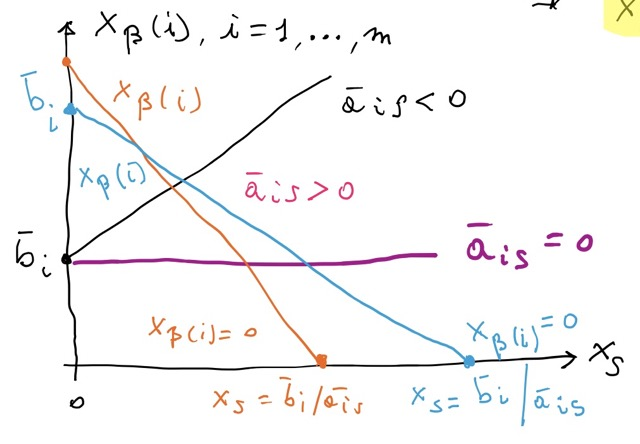
\includegraphics[scale=0.4]{bi.jpeg}
		\caption{Possibilità con i valori di $\overline{a}_{is}$} 
		\label{bi}
		\end{figure}


		Per \hl{$\overline{a}_{is} > 0$} avremo che ad un certo punto \hl{$x_s$ arrivera' a 0}. Ma potrebbe capitare che ci sia \hl{un'altra variabile che diventi 0 prima}, per un valore inferiore di $x_s$.

		Per \hl{esempio} se abbiamo una f.o.:
		$$\min z = -10x_1 - 10x_2 + 0$$

		vincoli:
		\begin{itemize}
			\item $2x_1 + x_2 + x_3 = 10$
			\item $x_1 + 2x_2 + x_4 = 10$
			\item $x_1, x_2, x_3, x_4 \geq 0$\\
		\end{itemize}

		BFS:
		\begin{itemize}
			\item $x_1 = x_2 = 0$
			\item $x_3 = 10$
			\item $x_4 = 10$
			\item $\hat{z} = 0$\\
		\end{itemize}

		\hl{allora}:
		$$x_s = \text{argmin} (-10, -10) = x_1$$

		annullando $x_2$, $x_3$, $x_4$:
		$$x_2 \leq \min (\frac{10}{2}, \frac{10}{1}) = 5$$

		il che significa che $x_s = x_1$, ed abbiamo:
		$$x_3 = 10 - 2x_1 \geq 0$$
		$$x_4 = 10 - x_1 \geq 0$$

		allora abbiamo:


		\begin{figure}[H]
		\centering
		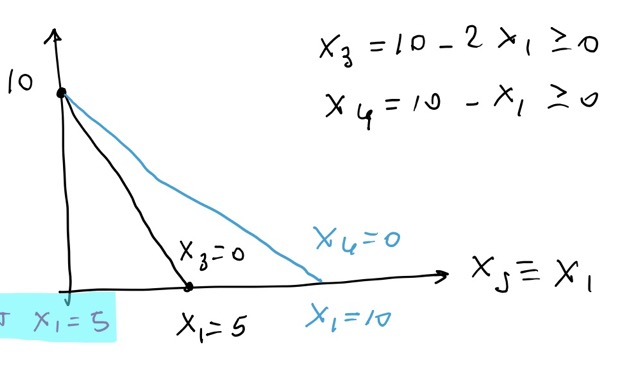
\includegraphics[scale=0.4]{disc.jpeg}
		\caption{Permutazione di $x_1$} 
		\label{disc}
		\end{figure}


		Dopo la nostra perturbazione $x_1 = 0 \to\ 5$ e $x_3 = 10 \to\ 0$, per determinare quale sia la \hl{variabile, detta variabile uscente, che si annulla per prima}:

		$$x_r = \text{argmin} (\frac{10}{2}, \frac{10}{1}) = x_3$$

\end{enumerate}

Lo \hl{pseudocodice} sarà:

\begin{enumerate}
	\item prendere una \hl{BFS}: $x_{BFS}$
	\item in un loop mentre $\exists\ \overline{c}_j \leq 0\ \ \ \forall\ \ \ j \in I_N$:
		\begin{itemize}
			\item $x_s = \text{argmin}_{j \in I_N} \overline{c}_j$
			\item se $\overline{a}_{is} \leq 0\ \ \ \forall\ \ \ i = 1, ..., m$ fa return del problem unbounded
			\item altrimenti $x_2 = \text{argmin} \frac{\overline{b}_i}{\overline{a}_{is}}\ \ \ \forall\ \ \ i = 1, ..., m;\ \overline{a}_{is} > 0$ detta variabile uscente
			\item makePivot(r, s) sennò non posso fare il test di ottimalità una volta reiniziato il loop
		\end{itemize}
\end{enumerate}


% Esercizio forma canonica
\subsection{Esercizio forma canonica}

Funzione obiettivo:

$$\max z = 10x_1 + 10x_2$$

vincoli:

\begin{itemize}
	\item $2x_1 + x_2 \leq 10$
	\item $x_1 + 2x_2 \leq 10$
	\item $x_1, x_2 \geq 0$
\end{itemize}

gradiente:

$$\nabla z =
\left[ {\begin{array}{c}
	10 \\
	10 \\
\end{array} } \right]
$$

grafico:

\begin{figure}[H]
\centering
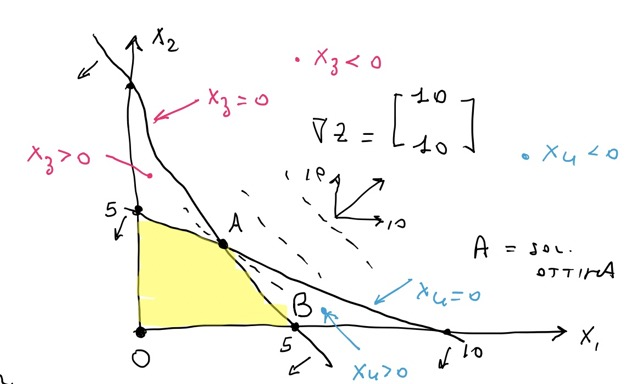
\includegraphics[scale=0.4]{grafescan.jpeg}
\caption{Graficazione dei vincoli} 
\label{grafescan}
\end{figure}

Forma standard:

$$\min z = -10x_1 - 10x_2$$

vincoli:

\begin{itemize}
	\item $2x_1 + x_2 + x_3 = 10$
	\item $x_1 + 2x_2 + x_4 = 10$
	\item $x_1, x_2, x_3, x_4 \geq 0$
\end{itemize}

avremo che:

\begin{itemize}
	\item $A = (3.\overline{3}, 3.\overline{3}, 0, 0)$
	\item $B = (5, 0, 0, > 0)$
	\item $O = (0, 0, > 0, > 0)$
\end{itemize}

dove nei vertici abbiamo \hl{2 variabili $> 0$}. Quindi ad ogni vertice abbiamo una BFS con \hl{cardinalita' $1:M$}.

Tableau:

$$
\left[ {\begin{array}{ccccc}
	2 & 1 & 1 & 0 & 10\\
	1 & 2 & 0 & 1 & 10\\
	-10 & -10 & 0 & 0 & 0\\
\end{array} } \right]
$$

con \hl{variabili} in base $B$ e non in base $N$:

\begin{itemize}
	\item $J_B = <X_3, x_4>$
	\item $J_N = <X_1, x_2>$
\end{itemize}

BFS:

\begin{itemize}
	\item $x_1 = x_2 = 0$
	\item $x_3 = 10$
	\item $x_4 = 10$
	\item $\overline{z} = 0$
\end{itemize}

Il \hl{test di ottimalita' fallisce} e quindi possiamo avere una soluzione migliore. Applico l'\hl{euristica del valore di costo ridotto}. Sceglo a caso $x_s = x_1$.

Prendiamo la \hl{colonna $x_1$ e in base al valore unitario} presente in $x_3$ e $x_4$ allora avremo:
$$\min (\frac{10}{2}, \frac{10}{1}) = 5$$

\hl{non posso avere che $x_3 > 5$} dato che si deve fermare per non diventare negativo, cioè non ammissibile, dato che superiamo in punto $B$.

Allora dato che \hl{$x_3 = 0$ e $x_1$ prende il suo posto} avremo che le \hl{variabili di base cambiano} in:
$$J_B = <x_1, x_4>$$

Dobbiamo allora effettuare un'\hl{operazione di Pivot}:

\begin{itemize}
	\item divido per $2$ la riga 1:
		$$
		\left[ {\begin{array}{ccccc}
			1 & 0.5 & 0.5 & 0 & 5\\
			1 & 2 & 0 & 1 & 10\\
			-10 & -10 & 0 & 0 & 0\\
		\end{array} } \right]
		$$

		\item moltiplico per $-1$ la prima riga e poi sommo alla seconda:
		$$
		\left[ {\begin{array}{ccccc}
			1 & 0.5 & 0.5 & 0 & 5\\
			0 & 1.5 & -0.5 & 1 & 5\\
			-10 & -10 & 0 & 0 & 0\\
		\end{array} } \right]
		$$

		\item moltiplico per $-10$ la prima riga e poi sommo alla terza:
		$$
		\left[ {\begin{array}{ccccc}
			1 & 0.5 & 0.5 & 0 & 5\\
			0 & 1.5 & -0.5 & 1 & 5\\
			0 & -5 & 5 & 0 & 50\\
		\end{array} } \right]
		$$
\end{itemize}

allora abbiamo che la \hl{soluzione di base ammissibile} (BFS) è:

\begin{itemize}
	\item $x_2 = x_3 = 0$
	\item $x_1 = 5$
	\item $x_4 = 5$
	\item $\overline{z} = -50$
\end{itemize}

Nuovamente il test di \hl{ottimalita' fallisce} per la presenza di $-5$, quindi la variabile entrante è $x_s = x_2$ quindi:
$$x_r = \text{argmin} (\frac{5}{0.5}, \frac{5}{1.5}) = x_4$$

il che corrisponde a stare in $B$ dove $x_2 = 0$, quindi ci spostiamo in direzione di $A = (> 0, > 0, 0, 0)$. Avremo allora:
$$J_B = <x_1, x_2>$$

dato che abbiamo \hl{$x_2$ entrante e $x_4$ uscente}.

Il perno del nuovo \hl{Pivot} sarà $1.5$:

$$
\left[ {\begin{array}{ccccc}
	1 & 0 & 0.\overline{6} & -0.\overline{3} & 3.\overline{3}\\
	0 & 1 & -0.\overline{3} & 0.\overline{6} & 3.\overline{3}\\
	0 & 0 & 3.\overline{3} & 3.\overline{3} & 66.\overline{6}\\
\end{array} } \right]
$$

avremo allora: 
\begin{itemize}
	\item $x_3 = x_4 = 0$
	\item $x_1 = 3.\overline{3}$
	\item $x_2 = 3.\overline{3}$
	\item $\overline{z} = -66.\overline{6}$
\end{itemize}

dove abbiamo ottenuto una \hl{soluzione ottima}.


% Soluzioni ottime multiple
\subsection{Soluzioni ottime multiple}

Per individuarle ricordiamo che esiste una soluzione ottima se: 

$$\overline{c_j} \geq 0$$

\hl{esistono soluzioni multiple se esiste $j^{*} \in J_N$} e quindi se ha:

\begin{itemize}
	\item \textbf{coefficienti di costo} ridotti $> 0$
	\item coefficienti delle \textbf{varibiali non di base} sono $> 0$
\end{itemize}

allora \hl{almeno uno sara' $= 0$}. Facendo il solito ragionamento \hl{prendo una variabile $x_{j*} = 0 \to\ > 0$}, allora avrò che:

$$\Delta z = \overline{c}_{j*} x_{j*} = 0$$


% Esempio soluzioni ottime multiple
\subsection{Esempio soluzioni ottime multiple}

Funzione obiettivo:

$$\max z = 20x_1 + 10x_2$$

vincoli:

\begin{itemize}
	\item $2x_1 + x_2 \leq 10$
	\item $x_1 + 2x_2 \leq 10$
	\item $x_1, x_2 \geq 0$
\end{itemize}

gradiente:

$$\nabla z =
\left[ {\begin{array}{c}
	20 \\
	10 \\
\end{array} } \right]
$$

grafico:

\begin{figure}[H]
\centering
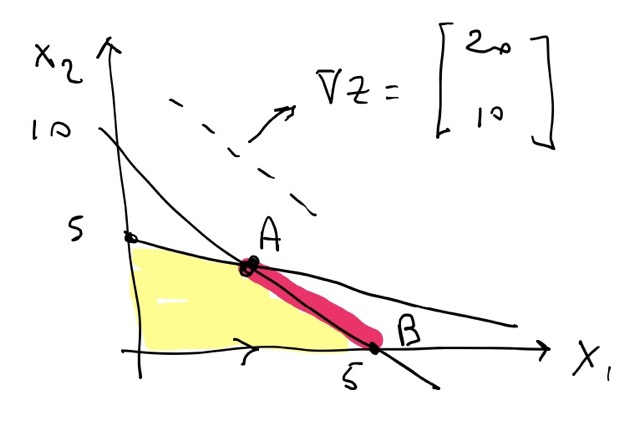
\includegraphics[scale=0.4]{grafsolmult.jpeg}
\caption{Graficazione dei vincoli} 
\label{grafsolmult}
\end{figure}

tableau:

$$
\left[ {\begin{array}{ccccc}
	2 & 1 & 1 & 0 & 10\\
	1 & 2 & 0 & 1 & 10\\
	-20 & -10 & 0 & 0 & 0\\
\end{array} } \right]
$$

BFS:

\begin{itemize}
	\item $x_1 = x_2 = 0$
	\item $x_3 = 10$
	\item $x_4 = 10$
	\item $\overline{z} = 0$
\end{itemize}

Usiamo le operazioni di Pivot:

$$
\left[ {\begin{array}{ccccc}
	1 & 0.5 & 0.5 & 0 & 5\\
	0 & 1.5 & -0.5 & 1 & 5\\
	0 & 0 & 10 & 0 & 100\\
\end{array} } \right]
$$

BFS:

$$B =
\begin{cases} 
    x_2 = x_3 = 0 \\ 
    x_1 = 5 \\
	x_4 = 5 \\
	\overline{z} = -100
\end{cases}
$$

Il \hl{test di ottimalita'} sulle variabili non di base $J_N = <x_2, x_3>$ è OK, \hl{ma non e' una soluzione unica} dato che \hl{abbiamo $0$ per $x_2$} che andrà \hl{perturbata} assegnandole un valore $> 0$. Allora la variazione della funzione obiettivo per una perturbazione è:
$$\overline{c}_{j*}x_{j*}\ \ \ \forall\ \ \ \overline{c}_{j*}=0,\ x_{j*} > 0$$

allora \hl{lungo lo spigolo $\overline{AB}$ avremo un costo minimo}. \hl{Forziamo il Pivot in $x_2$} facendo uscire $x_4$:

$$
\left[ {\begin{array}{ccccc}
	1 & 0 & 0.\overline{6} & -0.\overline{3} & 3.\overline{3}\\
	0 & 1 & -0.\overline{3} & -0.\overline{6} & 3.\overline{3}\\
	0 & 0 & 10 & 0 & 100\\
\end{array} } \right]
$$

BFS:


$$A =
\begin{cases} 
    x_3 = x_4 = 0 \\ 
    x_1 = 3.\overline{3} \\
	x_2 = 3.\overline{3} \\
	\overline{z} = -100
\end{cases}
$$

Abbiamo generato i due punti estremi $A$ e $B$ riuscendo ad avere \hl{infinite soluzioni ottime} dato che ci muoveremo nel segmento $\overline{AB}$. Al massimo potrenno essere:

$$\binom{n}{m}$$ 


% Algoritmo della convergenza
\subsection{Algoritmo della convergenza}

Abbiamo che \hl{se $c_s$ e' la varibiale entrante} allora il costo è dato dalla relazione:

$$\Delta z = \overline{c}_s \min_{i = 1, ..., m}\frac{\overline{b}_i}{\overline{a}_{is}}\ \ \ \forall\ \ \ \overline{a}_{is} > 0$$

con $\overline{c}_s < 0$ e $\min_{i = 1, ..., m}\frac{\overline{b}_i}{\overline{a}_{is}} \geq 0$


L'algoritmo del simplesso \hl{si comporta in modo decrescete} e ad ogni iterazione \hl{genera una nuova BFS}. Se ad ogni iterazione $\Delta z < 0$ vuol dire che avremo come \hl{casi sfavorevoli}:

\begin{itemize}
	\item \hl{$\min < 0$}: l'algoritmo visita tutte le BFS
	\item \hl{$\min = 0$}: uno dei numeratori è nullo
\end{itemize}

Se abbiamo che $x_s = 0$ esisterà un termine noto $\overline{b}_i = 0$ per $\overline{a}_{is} > 0$.

Avremo allora che \hl{se non abbiamo variazioni di $z$} allora \hl{non ci sara' un miglioramento}, dato che l'algoritmo è deterministico genererò la stessa sequenza all'infinito. Questo fenomeno è detto \hl{cycling} e avremo che l'algoritmo non converge.


\begin{figure}[H]
\centering
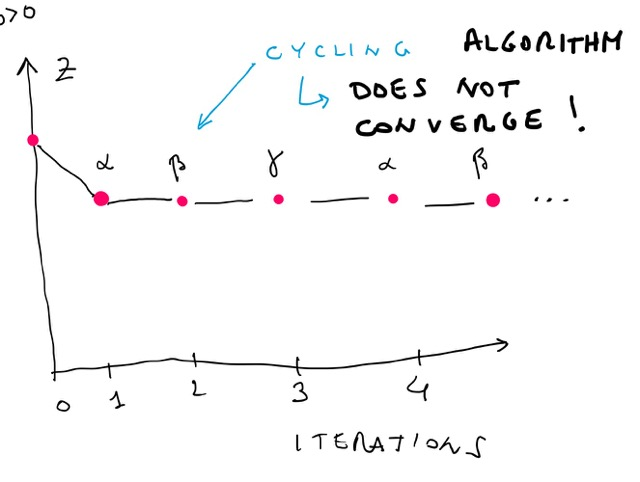
\includegraphics[scale=0.3]{notconv.jpeg}
\caption{Cycling algorithm result} 
\label{notconv}
\end{figure}
	

Potrebbe anche capitare di \hl{avere un miglioramento dopo $n$ iterazioni}.


\begin{figure}[H]
\centering
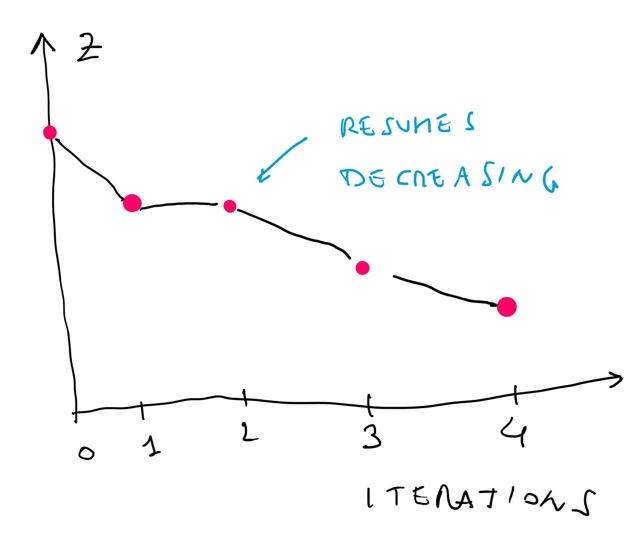
\includegraphics[scale=0.3]{conv.jpeg}
\caption{Not cycling algorithm result} 
\label{conv}
\end{figure}
		
	
% Esempio BFS degenere
\subsection{Esempio BFS degenere}

Funzione obiettivo:
$$\max z = 10x_1 + 10x_2$$

vincoli:

\begin{itemize}
	\item $x_1 - x_2 \leq 0$
	\item $x_2 \leq 1$
	\item $x_1, x_2 \geq 0$
\end{itemize}

grafico:


\begin{figure}[H]
\centering
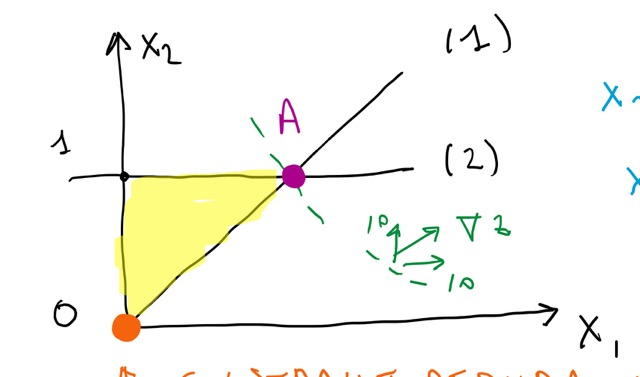
\includegraphics[scale=0.3]{esdegen.jpeg}
\caption{Grafico di un sistema inizialmente degenere} 
\label{esdegen}
\end{figure}

tabelau:

$$
\left[ {\begin{array}{ccccc}
	1 & -1 & 1 & 0 & 0\\
	0 & 1 & 0 & 1 & 1\\
	-10 & -10 & 0 & 0 & 0\\
\end{array} } \right]
$$

dove $\Delta z = 0 * x_1 = 0 * 0 = 0$

Notiamo di avere una variabile in base $= 0$ che sarà detta \hl{variabile degenere}. Dato che abbiamo dei termini negativi, nell'ultima riga, allora \hl{prendiamo quello con numero piu' negativo}, in questo caso anche con l'\hl{indice piu' negativo}$x_s = x_1$, allora:

$$x_r = \text{argmin} (\frac{0}{1}) = x_3$$

con $x_1 \leq \min (\frac{0}{1}) = 0$

Notiamo che abbiamo preso $x_3$ dato che \hl{in corrispondenza del numero piu' grande} abbiamo il valore unitario della colonna di $x_3$. 

Abbiamo un'altra soluzione degenere quindi ci troviamo su un \hl{plateau}. Graficamente abbiamo che $x_1$ rimane 0 nel punto $(0,0)$, avremo allora che nel segmento $\overline{0A}$ ci sarà un \hl{numero ridondante e superfluo di vincoli}. 


$$
\left[ {\begin{array}{ccccc}
	1 & -1 & 1 & 0 & 0\\
	0 & 1 & 0 & 1 & 1\\
	0 & -20 & 10 & 0 & 0\\
\end{array} } \right]
$$


Dove seguendo i motivi detti prima avremo $x_s = x_2$, allora:

$$x_r = \text{argmin}(\frac{1}{1}) = x_4$$

con $x_2 \leq \min(\frac{1}{1}) = 1$

Abbiamo quindi che:
$$\Delta z = -20 * x_2 = -20 * 1 = -20$$

prendendo come perno il valore più alto della colonna $x_2$ avremo un miglioramento:


$$
\left[ {\begin{array}{ccccc}
	1 & 0 & 1 & 1 & 1\\
	0 & 1 & 0 & 1 & 1\\
	0 & 0 & 10 & 20 & 20\\
\end{array} } \right]
$$

quindi con $\Delta z = - 20$.


% Regola dell'anticycling: Bland rule
\subsection{Regola dell'anticycling: Bland rule}

Possiamo \hl{evitare di avere variabili degeneri} usando la Bland Rule. Andremo semplicemente, \hl{a parita' di valore}, a prendere quello con \hl{indice piu' negativo}. Quindi in:


% Variabili artificiali
\subsection{Variabili artificiali}

Iniziamo aggiungendo \hl{ad ogni vicolo} una variabile artificiale:
$$\sum_j a_{ij}x_j + \alpha_i = b_i\ \ \ \forall\ \ \ i = 1, ..., m$$

con $\alpha_i \geq 0\ \ \ \forall\ \ \ i = 1, ..., m$.

Indicato con \hl{$P_a$ il problema artificiale}, la sua \hl{regione ammissibile sara'}:
$$\Omega(P_a) = \{\underline{x} \in R^m : \underline{\underline{A}}\ \underline{x} + \underline{\alpha} = \underline{b},\ \underline{x} \geq 0,\ \underline{\alpha} \geq 0,\ \underline{\alpha} \in R^m\}$$

Invece per il \hl{problema di partenza $P$}, la regione ammissibile è:
$$\Omega(P) = \{\underline{x} \in R^m : \underline{\underline{A}}\ \underline{x} = \underline{b},\ \underline{x} \geq 0\}$$

Avremo allora che:
$$\Omega(P_a) \geq \Omega(P) \Leftrightarrow x \in \Omega(P) \Rightarrow x \in \Omega(P_a)$$

La soluzione \hl{potrebbe comunque non essere ammissibile} per $P$. Allora cerchiamo una soluzione quivalente ma che sia valida sia per $P_a$ che per $P$.

Il problema artificiale (teorema 1) avrebbe come \hl{funzione obiettivo}:
$$\min \rho = \underline{e}^T \underline{\alpha}\ \ \ \forall\ \ \ e = [1, ..., 1]$$

vincoli:

\begin{itemize}
	\item $\underline{\underline{A}}\ \underline{x} + \underline{\alpha} = \underline{b}$
	\item $\underline{x}, \underline{\alpha} \geq 0$
\end{itemize}

Notare che \hl{ammette sempre soluzioni ottime}.

Per il teorema 2 avremo che $P$ è \hl{ammissibile $\Leftrightarrow$ $P_a$ ha $\rho^* = 0$}.

Dati quesi 2 problemi avremo che per:

\begin{enumerate}
	\item \hl{$\rho^* > 0$}: il problema $P$ è \textbf{inammissibile}
	\item \hl{$\rho^* = 0$}: alla soluzione ottima $P_a$ \textbf{corrispone una BFS per $P$}
\end{enumerate}


% Metodo del simplesso in 2 fasi
\subsection{Metodo del simplesso in 2 fasi}

Per prima cosa risolviamo il $P_a$ con il metodo del simplesso. Se \hl{$\rho^* = 0$ usiamo la soluzione ottima di $P_a$} senza le variabili artificiali. Prenderemo poi la \hl{f.o. $z$ come BFS per $P$} e da questa applicare il metodo del simplesso. 


% Costruzione del problema artificiale
\subsection{Costruzione del problema artificiale}

Funzione obiettivo:
$$\min z = \sum_{j = 1}^n c_jx_j$$

vincoli:

\begin{itemize}
	\item $\sum_{j=1}^n a_{ij}x_j \leq b_i\ \ \ \forall\ \ \ i = 1, ..., m_1$
	\item $\sum_{j=1}^n a_{ij}x_j \geq b_i\ \ \ \forall\ \ \ i = m_1+1, ..., m_2$
	\item $\sum_{j=1}^n a_{ij}x_j = b_i\ \ \ \forall\ \ \ i = m_2+1, ..., m$
\end{itemize}

con $x_j \geq 0\ \ \ \forall\ \ \ j = 1, ..., m$.

Forma standard abbiamo che la funzione obiettivo:
$$\min z = \sum_{j = 1}^n c_jx_j$$

vincoli:

\begin{itemize}
	\item $\sum_{j=1}^n a_{ij}x_j + x_{n+i} = b_i\ \ \ \forall\ \ \ i = 1, ..., m_1$
	\item $\sum_{j=1}^n a_{ij}x_j - x_{n+i} = b_i\ \ \ \forall\ \ \ i = m_1+1, ..., m_2$
	\item $\sum_{j=1}^n a_{ij}x_j = b_i\ \ \ \forall\ \ \ i = m_2+1, ..., m$
\end{itemize}

con 

\begin{itemize}
	\item $x_j \geq 0\ \ \ \forall\ \ \ j = 1, ..., n$
	\item $x_{n+i} \geq 0\ \ \ \forall\ \ \ i = 1, ..., m_2$
\end{itemize}

Per fare in modo di avere un problema artificiale con il \hl{minor numero di variabili artificiali} dovremo:

\begin{enumerate}
	\item per \hl{$i = 1, ..., m_1$ NON aggiungiamo variabili artificiali}, dato che abbiamo quelle di slack
	\item per \hl{$i = m_2 + 1, ..., m$ aggiungo una variabile artificiale} per ogni vincolo
	\item per \hl{$i = m_1 + 1, ..., m_2$ aggiungo una $\alpha_0$} in ogni vincolo
\end{enumerate}

Indichiamo un l'\hl{indice $h(m_1+1 \leq h \leq m_2)$} t.c.:
$$h = \text{argmax}_i\{b_i,\ i = m_1+1, ..., m_2\}$$

\hl{Rimpiazziamo ogni vincolo $i \neq h$ con} un vincolo quivalente:
$$\sum (a_{hj} - a_{ij})x_j - x_{n+h} + x_{n+i} = b_n - b_i\ \ \ \forall\ \ \ i = m_1 + 1, ..., m_2,\ i \neq h$$

avremo allora:
$$\sum a_{hj}x_j - x_{n+h} + \alpha_0 = b_n$$
$$\sum a_{ij}x_j - x_{n+i} + \alpha_0 = b_i$$


% Esempio problema artificiale
\subsection{Esempio problema artificiale}

Funzione obiettivo:
$$\min z = 4x_1 + 5x_2$$

vincoli:

\begin{itemize}
	\item $x_1 - x_3 = 6$
	\item $x_2 - x_4 = 4$
	\item $x_1 + 3x_2 = 21$
	\item $x_1, x_2, x_3, x_4 \geq 0$
\end{itemize}

Il problema artificiale è dato dalla funzione obiettivo:
$$\min \rho = \alpha_1 + \alpha_2$$

con vincoli:

\begin{itemize}
	\item $x_1 - x_3 + \alpha_1 = 6$
	\item $x_2 - x_4 + \alpha_1 = 4$
	\item $x_1 + 3x_2 + \alpha_2 = 21$
	\item $x_1, x_2, x_3, x_4, \alpha_1, \alpha_2 \geq 0$
\end{itemize}

Vado ora a \hl{sostituire al vincolo 2 la differenza tra il vincolo 1 e il 2}:
$$x_1 - x_2 - x_3 + x_4 = 2$$

Avremo allora che \hl{$P_a$ e' data da} una funzione obiettivo:
$$\min \rho = \alpha_1 + \alpha_2$$

e dai vincoli:

\begin{itemize}
	\item $x_1 - x_3 + \alpha_1 = 6$
	\item $x_1 - x_2 -x_3 + x_4 = 2$
	\item $x_1 + 3x_2 + \alpha_2 = 21$
	\item $x_1, x_2, x_3, x_4, \alpha_1, \alpha_2 \geq 0$
\end{itemize}

Applichiamo al \hl{prima fase del metodo a 2 fasi}:


$$
\left[ {\begin{array}{ccccccc}
	1 & 0 & -1 & 0 & 1 & 0 & 6\\
	1 & -1 & -1 & 1 & 0 & 0 & 2\\
	1 & 3 & 0 & 0 & 0 & 1 & 21\\
	0 & 0 & 0 & 0 & 1 & 1 & 0\\
\end{array} } \right]
$$

Per poter \hl{ripristinare la forma canonica} dovremo avere i \hl{coefficienti di $\alpha_1,\ \alpha_2 = 0$}. Tramite vari \hl{operazioni di Pivot} arriviamo a non avere più in base $\alpha_1$ e $\alpha_2$ facendo:
$$\text{f.o.} - \text{vincolo di }\alpha_1 - \text{vincolo di }\alpha_2$$

In fine avremo:


$$
\left[ {\begin{array}{ccccc}
	1 & 0 & -1 & 0 & 6\\
	0 & 0 & 0.\overline{3} & 1 & 1\\
	0 & 1 & 0.\overline{3} & 0 & 5\\
	0 & 0 & 2.\overline{3} & 0 & -49\\
\end{array} } \right]
$$

Avremo allora \hl{verificato il criterio di arresto}, perciò avremo una soluzione ottima:
$$x^* = (6, 5, 0, 1),\ z^* = 49$$


% Esercitazione variabili artificiali
\subsection{Esercitazione variabili artificiali}

Usando il metodo delle variabili artificiali, risolvere il seguente problema con funzione obiettivo:
$$\min z = 3x_1 - 7x_2 + 2x+3$$

con vincoli:

\begin{itemize}
	\item $2x_1 + 3x_2 + 5x_3 \leq 15$
	\item $x_1 + x_2 + x_3 \geq 1$
	\item $-x_1 + x_2 = 5$
	\item $x_1, x_2, x_3 \geq 0$
\end{itemize}

il problema in forma standard avrà come funzione obiettivo:
$$\min z = 3x_1 - 7x_2 + 2x+3$$

con vincoli:

\begin{itemize}
	\item $2x_1 + 3x_2 + 5x_3 + x_4 = 15$
	\item $x_1 + x_2 + x_3 - x_5 = 1$
	\item $-x_1 + x_2 = 5$
	\item $x_1, x_2, x_3 \geq 0$
\end{itemize}

Il problema artificiale è dato dalla funzione obiettivo:
$$\min \rho = \alpha_1 + \alpha_2$$

con vincoli:

\begin{itemize}
	\item $2x_1 + 3x_2 + 5x_3 + x_4 = 15$
	\item $x_1 + x_2 + x_3 - x_5 + \alpha_1 = 1$
	\item $-x_1 + x_2 + \alpha_2 = 5$
	\item $x_1, x_2, x_3, \alpha_1, \alpha_2 \geq 0$
\end{itemize}

Avremo allora:

$$
\left[ {\begin{array}{cccccccc}
	2 & 3 & 5 & 1 & 0 & 0 & 0 & 15\\
	1 & 1 & 1 & 0 & -1 & 1 & 0 & 1\\
	-1 & 1 & 0 & 0 & 0 & 0 & 1 & 5\\
	0 & 0 & 0 & 0 & 0 & 1 & 1 & 0\\
\end{array} } \right]
$$

Per ripristinare la forma canonica $\alpha_1$ e $\alpha_2$ devono essere $0$ facendo:
$$\text{f.o.} - \text{vincolo 2}$$

al risultato:
$$\text{risultato} - \text{vincolo 3}$$

$$
\left[ {\begin{array}{cccccccc}
	2 & 3 & 5 & 1 & 0 & 0 & 0 & 15\\
	1 & 1 & 1 & 0 & -1 & 1 & 0 & 1\\
	-1 & 1 & 0 & 0 & 0 & 0 & 1 & 5\\
	0 & -2 & -1 & 0 & 1 & 0 & 0 & -6\\
\end{array} } \right]
$$

Non essendo una soluzione ottima \hl{entriamo in base $x_2$} ($s = 2$):
$$\min (\frac{15}{3}, \frac{1}{1}, \frac{5}{1}) = 1$$

quidni abbiamo $r = 2$ facendo uscire $\alpha_1$. Facendo il Pivot abbiamo:

$$
\left[ {\begin{array}{cccccccc}
	-1 & 0 & 2 & 1 & 3 & -3 & 0 & 12\\
	1 & 1 & 1 & 0 & -1 & 1 & 0 & 1\\
	-2 & 0 & -1 & 0 & 1 & -1 & 1 & 4\\
	2 & 0 & 1 & 0 & -1 & 2 & 0 & -4\\
\end{array} } \right]
$$

che non e1 ottima. Entra in base $x_5$:
$$\min (\frac{12}{3},\ \frac{4}{1}) = 4$$

Notiamo che, avendo valori uguali, ci conviene prendere $r = 3$ in modo che se ne vada $\alpha_1$:

$$
\left[ {\begin{array}{ccccccc}
	0 & 0 & 1 & 0.4 & 1 & -0.2 & 4\\
	0 & 1 & 1 & 0.2 & 0 & 0.4 & 5\\
	1 & 0 & 1 & 0.2 & 0 & -0.6 & 0\\
	0 & 0 & 0 & 0 & 0 & 1 & 0\\
\end{array} } \right]
$$

che e1 soluzione ottima per il problema artificiale.
\newpage
\section{Branch-and-Bound Technique for Solving Integer Programs}

% Principio di funzionamento dell'argoritmo Branch-and-Bound
\subsection{Principio di funzionamento dell'argoritmo Branch-and-Bound}

l'imoportanza dell'ottimizzazzione di questi problemi sono date da alcune considerazioni:

i nostri problemi sono lineari con variabli decisionali i vincoli sono lineare. ma c'e1 di diverso che alcune variabili non sono continue ma posso assumere solo valori di tipo intero a volte anche binerie qiuidni 0 o 1:

approcci da usare:

brute force:
abbaimo un problema con n variabili di tipo binario, sappiamo che le soluzioni ammissimisi e non sono $2^n$. un approccio di brute force consiste nel generare tutte le soluzioni e per ciascune verificare se i vincoli sono soddisfatti e se si calcolare i lvalore della misura di performance

es:
\dots

ma questo approccio e1 naive dato che non e1 compitazionalemte ammissibile.

approccio 2:
non so risolvere i problemi con le variabili intere, ma appossimo il problema a variabili intere e "rilasso" il vincolo di intergita1:

chiamo allora P  il problema:

\dots

nel rilassamento continuo notiamo che non abbiamo il vincolo di =0/1, invece le variabili sono contenute tra 0 <= x >= 1.

risolvendo il problema puo1 uscire un valore frazionario dato che potrebbe uscire esattamente la meta1. avremo allora un caso fortunato (soluzione ottima) lo e1 anche per entrambi i problemi, quidni abbiamo che la soluzione e1 quella di partenza


caso sfortunato: abbiamo delle variabili trazioniarie allora arrotondo 0.53 -> 1, 0.35 -> 0

dopo un arrotondamento la soluzione potrebbe comunque essere non ammissibile o non ottima. i rounding allora avranno $2^{n}$



altro approccio:
possiamo solstituire il vincolo di binarieta con quello ci continuita questa sostituizione porta ad una soluzione non lineare allora e1 un prbema di ottimizazione non lineare per il quale non si conoscono procedimenti risolutivi ottimi.



approccio branch-and-bound:
e1 detta tecnica di enumeramerazione perasiale

1. ci si procura una stima del valore della soluzione ottima che e1 ottenuta andando a rialssare il vinclo di integratia1 sulle veriabili intere. 

che relazione c'e1 tra il problema lineare con variabili intere P e quello rilassaro R(P) con variabili rese continue

il rilassamento posso risolverlo tramite una blackbox che lo risolve cioe1 che dice se il problem e1 inammissibile soluzione illimitata, mi da la soluzione ottima. 


1 caso: rilassamento di P e1 inammissibile. in questo caso il porblema P sara1 inammissiible datoche che R(P) contiene P:

img

2 caso: la blackbox ci dice che i lproblema e1 unbounded, allora si possono verificare i casi in cui:

es: $x_1 \leq 0.5$

img

dove avremo sempre intersezioni con il regime ottimo, allora z tente a + infinito anche per quanto riguarda le variabili intere.

allora trovo che per R(P) unbounded avro1 P unbounded o non ammissibile:

es: $x_1 \geq \frac{1}{3},\ x_1 \leq \frac{2}{3}$

img

allora non avremo delle variaibli intere




stiamo allora cercando di risolver il problema P a variaibli intere tramite il suo rilassamento.

3 caso: abbiamo la soluzione ottima, ma:

1. potrebbe capitare che il rilassamento R(P) ha soluzione ottima ma e1 inammissible P:

es:

img

2. abbiamo f.o:

vincoli:

img

avremo come soluzioni intere 0,0 0,1 1,0 quindi il rilassamento e1 ammissibile ma se gaurdiamo le soluzioni ottime 


vado a traslare la curva di livello fino a trovare la soluzione R(P) data dal primo punto ammissibile del quadrante. per la soluzione ottima di P dobbiamo prendere la prima soluzione ocntinua


avremo come soluizione ottima di ottimizzazione sempre quella di R(P) quindi quella del rilassamento continuo dato che ha meno vincoli quindi fornisce una soluzione ottimistica, cioe1 che ci da1 una soluzione miglioe o ugulae della nostra stima. quindi ci fornisce una stima per eccesso


quindi in ogni caso la soluzione ottima del problema se stiamo massimizzando e1 sempre sovfrastata dalla soluzojne ottiam del continuo. se sto massimizzando allora la soluzione ottiam continua e1 maggiore = ottima della solzioine ottima a variaibli intere se sto minimizzando ragiono al contrario



ma notiamo che se risolvo il rilassamento che mi viene dato dalla black box non posso sapere se il problema P e1 unbounded o non ammissibile.

poi abbiamo capiteo che poiche1 c'e1 l'ambiguita1 e non so cosa sucede a P, oltre a conoscere il bounding si usa un branch cioe1 una suddivisione del problema in sottoproblemi. 

es: 

do alla blackbox il rilassamento dove abbiamoche ha soluzione ottima in 2.25, 3.75 con z = 41.25

sul problema P possi dire che se fosse ammissiible no avrebbe un valore di z superiore a 41.25 

sappiamoche se P ha soluzione ottiama non puo1 esserea superiore a 41.25


effetttuo allora un branch per creare dei sottoproblmi allora la soluzione si trova in uno die due. la nostra soluzione e1 frazionaria, una soluzonedl problema a variabili intere o si trova in un sottoproblema o nellaltro:

sottoprob p1:\dots

sotttoprob P2:\dots


allora una soluzoone interea del porblema P si traova per forza in uno dei 2 sottoproblemi dato che nel gp tra i due non ci sono valori interi. allora
1 caratt: dividi il polema di partenza in sottoprob con una soluzoine ch ei strov ain p1 o p2 
2 careatt: il branch taglia la soluzione frazionario (scegliendo arbitrariamente $x_1$ o $x_2$)

img

ma in realta1 questi sotoproblemi sono insisemi di ammissibiilita del problema rilassato dei sottoproblemi


analizzando i due sottoproblemi abbiamo che al primo abiamo che risolvendo il sottoproblema 1 con soluzione 3, 3 con z = 39 allora non ho bisogno di eplorare ancora dato che ho gia1 la soluzione ottima:

img

dato che e1 intera la soluzione allora non devo piu1 cercarne nel sottoprob 1 (soluizone ammissible che possono implemntare che ha un oprfitto di 39 ma non sono certo ceh si a soluzione ottiam di tuto il porblema ma sicuro di quello p1)


in p2 invece abbiamo che la soluzione ottima del rilassamento e1 1.8, 4 z = 41 sone z e1 l'upperbound che e1 una stima per eccesso ottistica che limita le soluzioni.

arrestando ora l'algoritmo abbiamo che non potremo sapere se il secondo sottoproblema dara1 un valore migliore. dato che e1 una "promessa" posso arrivarci ma non e1 detto

se entrambe le sottopblb sono uguali e mi serve una sla soluzione posso fermarmi
\newpage
\section{Constructive heuristics}

% Introduzione
\subsection{Introduzione}
Nel (caso peggiore) di variabili binarie il livello computazionale sarà dato da $O(2^n)$ quindi il tempo di calcolo cresce esponenzialmente con il numero di variabili. 

In molte applicazioni si fa affidamento ad \hl{algoritmi detti inesatti} che \hl{CERCANO di generare delle soluzioni ammissibili}. Questi rientrano negli \hl{algoritmi euristici} dove è importante che la \hl{conoscenza del progettista venga trasmessa all'algoritmo}. Questi algoritmi possono essere:

\begin{itemize}
    \item \textbf{costruttivi}: dove \hl{cercano di generare una prima soluzione ammisibile}
    \item \textbf{migliorativi}: dove \hl{prova a migliorare la prima soluzione}
\end{itemize}

Trovare una soluzione ammissibile potrebbe essere difficile dato che potrebbe essere più complicato del trovarne una ottima.


% Travellig Salesman Problem (TSP)
\subsection{Travellig Salesman Problem (TSP)}

Data una matrice $C$ di transizione dove, per andare dal punto $1$ al $2$ \hl{pago $c_{12}$} e così via per tutte le possiabili iterazioni \hl{per un numero $n$ di punti da "visitare"}. Lo scopo sarebbe trovare un circuito che tocchi tutti i punti una sola volta con \hl{costo minimo}.

Avremo che il \hl{tempo di ciclo determina la produttivita' della macchina} tipo un robot che fa n fori e conclusi gli n fori finisce oil cilo.

Un vincolo ulteriore potrebbero essere le \hl{finestre temporali} che potrebbero esserci come nei casi di consegna dei pacchi amazon, il che \hl{rende computazionalmente piu' difficile o anche inammissibile il problema}. Notare come cambiando anche solo un dato potremmo avere una soluzione ammsisibile o una crescita esposnenziale dell'infattibilità dala quele deriva l'instabilità.


% Algoritmo greedy
\subsection{Algoritmo Greedy}

Algoritmo che \hl{cerca di massimizzare nel breve periodo} (usato per essere adattato a qualsiasi problema). È un'\hl{euristica di tipo costruttivo}, infatti ha una \hl{procedura sequenziale} che costruisce la soluzione passo passo \hl{massimizzando solo l'utilizzo immediato} andando però in contro a:

\begin{itemize}
    \item una soluzione inammissibile
    \item non garantire una soluzione ottima
\end{itemize}

il suo \hl{pseudocodice} è un adattamenteo sull'algoritmo del Travellig Salesman Problem (TSP):

\begin{itemize}
    \item[] last = 1 (last = ultimo punto toccato)
    \item[] $S = \{2,3,...,n\}$
    \item[] while ($S \neq$ insieme vuoto)
    \begin{itemize}
        \item[] estrarre da $S$ un punto
        \begin{itemize}
            \item[] $i = \text{argmin}_{i \in S} c_{\text{last}, i}$
            \item[] $\text{succ}_{last} = i$
            \item[] last $= i$
        \end{itemize}
    \end{itemize}
    \item[] $\text{succ}_{last} = 1$ 
\end{itemize}

Vediamo un esempio con dati: $n = 4$ e
$$C=
\left[ {\begin{array}{cccc}
    0 & 10 & 5 & 8 \\
    10 & 0 & 2 & 1 \\
    5 & 2 & 0 & 4 \\
    8 & 1 & 4 & 0 \\
\end{array} } \right]
$$

dove applicando l'algoritmo abbiamo:

\begin{itemize}
    \item last = 1; $\rho = <2,3,4>$
    \item last = 3 ; $\rho=<2,4>$; $\text{succ}_1 = 3$
    \item last = 2; $\rho=<4>$; $\text{succ}_3 = 2$
    \item last = 4; $\rho =<>$; $\text{succ}_2 =4$
    \item $\text{succ}_4 = 1$
\end{itemize}


% Miller-Tucker-Zemlin
\subsection{Miller-Tucker-Zemlin}

Questo modello definisce delle \hl{variabili binare $x_{ij}$} per ogni coppia di punti $i$ e $j$:

$$ x_{ij} =
\begin{cases} 
    1, \text{ se } i,\ j \text{ sono/saranno visitati} \\ 
    0, \text{altrimenti}
\end{cases}
$$

avremo allora che:
$$\min \sum_{i,j} c_{i,j} x_{i,j}$$
s.t
\begin{itemize}
    \item $\sum{j} x_{ij} = 1\ \ \ \forall i$
    \item $\sum{j} x_{ji} = 1\ \ \ \forall i\ ->$ dice che ogni punto ha un suo successore
    \item $0 \leq x_{ij} \leq 1\ \ \ \forall x_{ij} \text{ integer} ->$ dice ogni punto ha un predecessore
\end{itemize}

Questi \hl{vincoli non bastano} per poter risolvere il modello, infatti non possiamo escludere di avere una \hl{soluzione disconnessa (sub-tour)}


\begin{figure}[H]
\centering
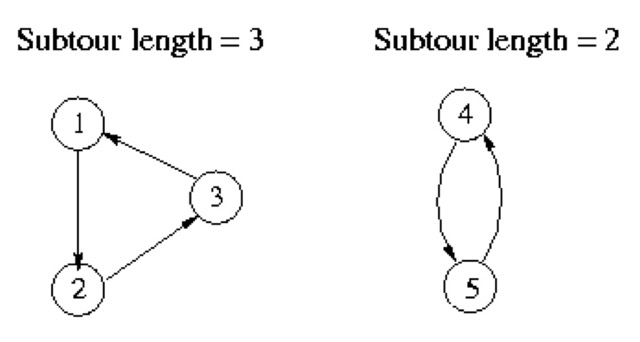
\includegraphics[scale=0.3]{sep.jpeg}
\caption{Soluzione disconnessa} 
\label{sep}
\end{figure}


Si introducono allora dei \hl{vincoli di connessione} della soluzione tramite una \hl{variabile per l'ordine di vista: $u_i$} (una per ogni punto).

Poniamo allora un punto iniziale con $u_i = 1$:

\begin{itemize}
    \item[] $u_1 = 1 -> x_{1,3} = 1$
    \item[] $u_3 = 2 -> x_{3,4} = 1$
    \item[] $u_4 = 3 -> x_{4,2} = 1$
    \item[] $u_2 = 4 -> x_{2,1} = 1$
\end{itemize}

altri \hl{vincoli da imporre su $u_i$}:

\begin{itemize}
    \item $2 \leq u_i \leq 1\ \ \ \forall i \neq 1$
    \item $u_i - u_j + 1 <= n(1-x_{ij})\ \ \ \forall i,j \neq 1$
\end{itemize}

Avremo quidni \hl{2 casi}:

\begin{itemize}
    \item $x_{ij} = 0\ \Rightarrow\ u_i - u_j +1 \leq n$: ovvio dato che tutte le variabili \textbf{$u$ sono comprese in $n$}
    \item $x_{ij} = 1\ \Rightarrow\ u_i - u_j + 1 \leq 0$: dato che $u_j \geq u_i + 1$ allora \textbf{$i$ predecessore di $j$}
\end{itemize}


% Algoritmo relax-and-fix
\subsection{Algoritmo relax-and-fix}

Si usa per \hl{problemi multiperiodali} dato che voglio poter avere un approccio con \hl{suddivisione in piu' periodi temporali}:

$$\min z = c^Tx$$
s.a.
\begin{itemize}
    \item $Ax=b$
    \item $x \geq 0$ (integer)
\end{itemize}

\hl{Partiziono le variabli in $n$ gruppi} in modo da avere variabili impiegate per un solo intervallo di tempo. Allora il problema diventa:

abbiamo alloradelle applicazioni ndove le varaibili naturalemte si dividono in gruppi datoun osviluppo temporale, il orblema allora diventa:

$$\min z = \sum_{i=1}^n c_i^Tx_i$$
s.a.
\begin{itemize}
    \item $\sum_{i=1}^na_ix_i=b$
    \item $x_i \geq 0$ (integer)
\end{itemize}

la difficoltà del problema si trova nelle molte varibili intere. Posso allora \hl{definire un problema con variaibli $x_1$ del primo gurppo intere}, per le restanti faccio un rilassamento. Potremo avere che:


\begin{itemize}
    \item ausiliario: inammissibile $\to$ iniziale: inammissibile
    \item ausiliario: sol. ottima $\to$ fisso $x_1$ alla soluzione: $x_1 = \overline{x}_1$
\end{itemize}

Quindi per \hl{risolvere il problema} dobbiamo:

\begin{enumerate}
    \item $\underline{x}_1$ diventa \textbf{intera}
    \begin{itemize}
        \item \textbf{rilasso} le altre variabili
        \item \textbf{risolvo} il problema e \textbf{fissiamo} $x_1 = \overline{x}_1$ che viene "rimossa" dal modello
    \end{itemize}

    \item ecc, ecc...
\end{enumerate}

Così facendo \hl{tengo conto delle variabili "future"} senza richiede un grande sforzo computazione, dato che lavora sul singolo gruppo.

\hl{Generallizzando}:
$$\min x = \sum_{i=1}^{k-1} c_i \overline{x}_i + c_k x_k + \sum_{i=k+1}^n c_i x+i$$
s.t

\begin{itemize}
    \item $\sum_{i=1}^{k-1} a_i \overline{x}_i + a+k x+k + \sum_{i=k+1}^n a_i x_i = b$
    \item $x_k \geq 0$ (integer)
    \item $x_i \geq 0$
\end{itemize}

Lo \hl{pseudocodice} sarà:

\begin{itemize}
    \item[] found = true
    \item[] for (k = 1 $\to$ n):
    \begin{itemize}
        \item[] solve $P_k(\overline{x}_1,...,\overline{x}_{k-1})$
        \item[] if è inammissibile:
        \begin{itemize}
            \item[] found = false
            \item[] break;
        \end{itemize}
        \item[] else: $(x'_{k+1},...,x'_n)$ è soluzione
        fissare $\overline{x}_k = x'_{k}$
    \end{itemize}
\end{itemize}


% Algoritmo rolling horizon
\subsection{Algoritmo rolling horizon}

Durante il primo periodo considero di:

\begin{enumerate}
    \item creare un \hl{sottoproblema con alcune variabili} da $x_1$ a $x_k$
    \item \hl{trascurare le variabili dei periodi successivi}
    \item fisso $x_1$
    \item mi \hl{muovo di uno step}
    \item considero un \hl{sottoproblema con $x_1$}
    \item \hl{fisso $x_2$} e considero le variabili fino a $x_k+1$.
    \item ecc, ecc...
\end{enumerate}

Andiamo quindi a \hl{risolvere un problema a $k$ variabili} ma \hl{senza tenere in conto le variabili troppo successive}, quindi sarà meno accurato.


% Multiple criteria decision making
\subsection{Multiple criteria decision making}

Spesso abbiamo \hl{piu' obbiettivi} e \hl{non riusciamo a scegliere in anticipo quale ha priorita'} allora spesso vanno in \hl{conflitto}, allora cerchiamo di trovare le migliori soluzioni che devono \hl{rispettare alcuni vincoli}:

$$p \text{ criteria } =
\begin{cases} 
    z_1 = f_1(x) \text{ da }\min \text{ o }\max \\ 
    z_2 = f_2(x) \text{ da }\min \text{ o }\max \\ 
    ... \\
    z_p = f_p(x) \text{ da }\min \text{ o }\max
\end{cases}
$$
s.t

\begin{itemize}
    \item $g(x) \geq 0$
    \item $x \geq 0$
\end{itemize}


% Esempio problema scheduling
\subsection{Esempio problema scheduling}

Preso un problema di scheduling, abbiamo $n$ attività con paramentri:

\begin{itemize}
    \item $S_i$: starting time dell'attività $i$
    \item $d_i$: durata dell'attività $i$
    \item $p_{ij} = 1$ se l'attivtà $j$ è prerequinistito dell'attività $i$
    \item $p_{ij} = 0$ altrimenti
\end{itemize}

come f.o: $\min T$ con $T$ tempo di completamento:
$$\min T$$
s.t.

\begin{itemize}
    \item $T \geq S_i + d_i,\ i = 1, ..., n$
    \item $S_i \geq p_{ij} (S_j + d_j),\ i,j = 1, ..., n$
\end{itemize}

Per poter \hl{formulare un'attivita' in modo fattibile}:

\begin{itemize}
    \item $D_i$: max durata dell'attività $i$
    \item $b_i$: min durata dell'attività $i$
    \item $d_i$: durata dell'attività $i$
    \item $X_i$: costo per accellerare il completamento dell'attività $i$
\end{itemize}


allora:

\begin{itemize}
    \item $d_i = D_i-a_iX_i$ con $a_i$ coefficente in unità di tempo
    \item $d_i \geq b_i$
\end{itemize}

abbiamo da minimizzare 2 obiettivi:
$$min \sum_{i=1}^n X_i$$
$$min T$$
s.t.

\begin{itemize}
    \item $T \geq S_i + d_i\ \ \ \forall\ \ \ i$
    \item $S_i \geq p_{ij} (S_j + d_j)\ \ \ \forall\ \ \ i, j, i \neq j$
    \item $d_i \geq b_i\ \ \ \forall\ \ \ i$
    \item $d_i = D_i - a_i X_i\ \ \ \forall\ \ \ i$
\end{itemize}


% Superior solutions
\subsection{Superior solutions}

Preson un problema con \hl{piu' obiettivi} allora ne consideriamo uno con obiettivo singolo, allora \hl{rappresento i singoli obiettivi} nello spazio.

Presa una soluzione potremo trovarne una migliore ma solo \hl{se si trova nella zona ammissibile e che sia nella frontiera}, in caso contrario è detta \hl{utopia}.

\begin{figure}[H]
\centering
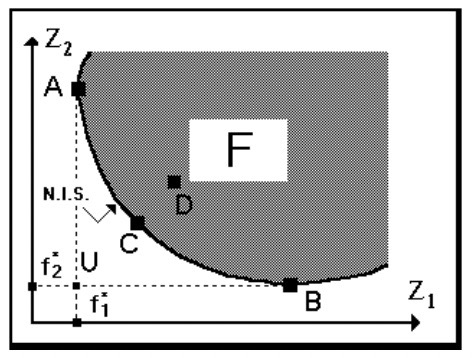
\includegraphics[scale=0.3]{utop.jpeg}
\caption{Utopia} 
\label{utop}
\end{figure}

Definiamo invece \hl{soluzione superiore} la soluzione che minimizza o massimizza meglio di tutte (come U se fosse nella zona ammissibile).

Si parla allora di soluzioni dominate e soluzioni non dominate (di \hl{Pareto}).

Per \hl{confrontare due soluzioni di Pareto} usiamo il \hl{trade-off ratio} tamite:

$$|\frac{z_i(x_A)-z_i(x_B)}{z_j(x_A)-z_j(x_B)}|$$

che rappresenta il \hl{miglioramento dell'obiettivo i-esimo in base al miglioramento di un altro obiettivo}.

Nel caso di una \hl{zona convessa} collegneremo i punti limite tramite una \hl{tangente immagginaria}, dalla quale però non prendere mo i punti di frontiera.

\begin{figure}[H]
\centering
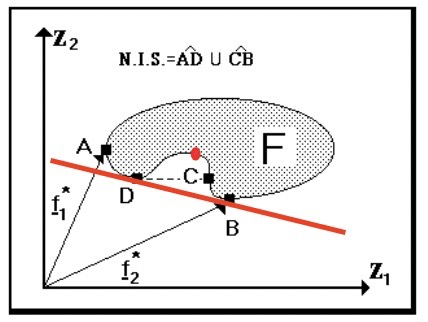
\includegraphics[scale=0.3]{convess.jpeg}
\caption{Zona convessa} 
\label{convess}
\end{figure}

per \hl{trovare le soluzioni efficenti} abbiamo 2 metodi:

\begin{enumerate}
    \item \hl{metodo dei vincoli}: \textbf{considero un solo obiettivo}, per gli altri avrò:
        $$\min f_i(x)$$
        
        s.t
        
        \begin{itemize}
            \item $f_k(x) \leq u_k$
            \item $g(x) \geq 0$
            \item $x \geq 0$
        \end{itemize}

        Prendo allora solo $A$ e $D$:

        \begin{figure}[H]
        \centering
        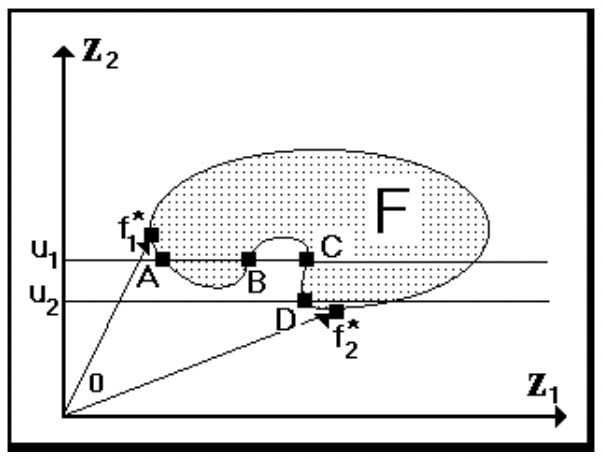
\includegraphics[scale=0.3]{vinc.jpeg}
        \caption{Metodo dei vincoli} 
        \label{vinc}
        \end{figure} 
    \item \hl{metodo dei pesi}: abbiamo una sola \textbf{f.o somma di tutti li obiettivi}:
        $$\min \sum_{i=1}^p w_i f_i (x)$$

        s.t
        
        \begin{itemize}
            \item $\sum_{i=1}^p w_i = 1$
            \item $g(x) \geq 0$
            \item $x \geq 0$
            \item $w_i \geq 0$
        \end{itemize}

        \begin{figure}[H]
        \centering
        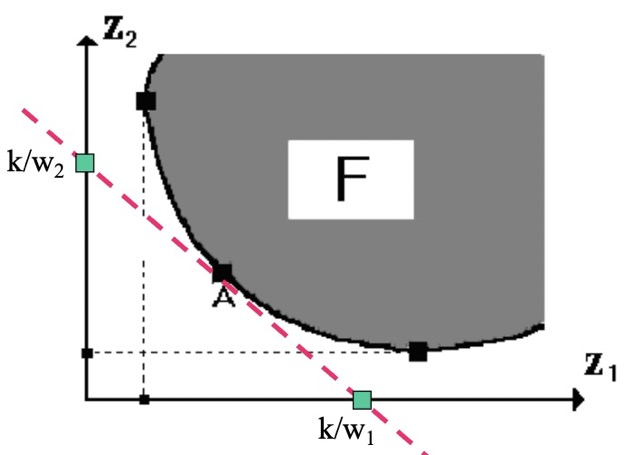
\includegraphics[scale=0.3]{pesi.jpeg}
        \caption{Metodo dei pesi} 
        \label{pesi}
        \end{figure}

        dove a seconda del valore che diamo ai pesi andiamo a \hl{spostare la retta trangente alla zona ammissibile}.
\end{enumerate}


% Metodo a priori
\subsection{Metodo a priori}

Per \hl{risolvere il singolo problema} usiamo:
$$\max U(f_1(x), f_2(x), ..., f_p(x))$$

s.t
\begin{itemize}
    \item $g(x) \geq 0$
    \item $x \geq 0$
\end{itemize}

ma in genere \hl{non si trova} questa soluzione.


% Metodo a posteriori
\subsection{Metodo a posteriori}

Generiamo tutte le \hl{soluzioni efficienti per dire quale e' la migliore}. Notare che così facendo si potrebbe avere una \hl{crescita esponenziale} del problema.

Una buona \hl{alternativa} è il metodo interattivo.


% Metodo interattivo
\subsection{Metodo interattivo}

Presi 2 obiettivi:

\begin{itemize}
    \item troviamo il \hl{punto ottimo per entrambi}
    \item troviamo la \hl{prima soluzione efficiente che sia tra $A$ e $C$}
    \item scegliere su \hl{quale parte della frontiera posizionarsi}
    \item ecc, ecc...
\end{itemize}

\begin{figure}[H]
\centering
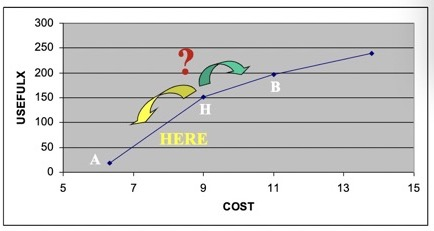
\includegraphics[scale=0.5]{intent.jpeg}
\caption{Metodo interattivo} 
\label{intent}
\end{figure}

mi fermerò quando il segmento che rimane è \hl{cosi piccolo che i due punti conincidono}.

\newpage
\section{Local Search}

% Introduzione
\subsection{Introduzione}

L'algoritmo di local search è di \hl{tipo euristico migliorativo}, cioè \textbf{presuppone che sia stata già prodotta una soluzione ammissibile}. 

Le \hl{procedure} da utilizzare si dividono in:

\begin{enumerate}
    \item \hl{single population}: \textbf{migliorare in un intorno (localmente) la situazione}, tenendo in conto che potrebbe rimanere bloccata in minimi locali
    \item \hl{multiple population}: ad ogni iterazione si ha un \textbf{insieme di soluzioni}
\end{enumerate}

Non essendo algoritmi precisi \hl{vanno adattati} al particolare problema che si intende affrontare.


% Progetto di ricerca locale
\subsection{Progetto di ricerca locale}

Si parte da una \hl{soluzione $x^{(0)}$} e si considera il suo \hl{intorno $N(x^{(0)}$}, cioè un \hl{insieme di soluzioni vicine a $x^{(0)}$} dove la definizione di "vicine" viene data dal progettista, aggiungiamo allora il vincolo:
$$\underline{x} \in N(\underline{x}^{(0)})$$


\begin{figure}[H]
\centering
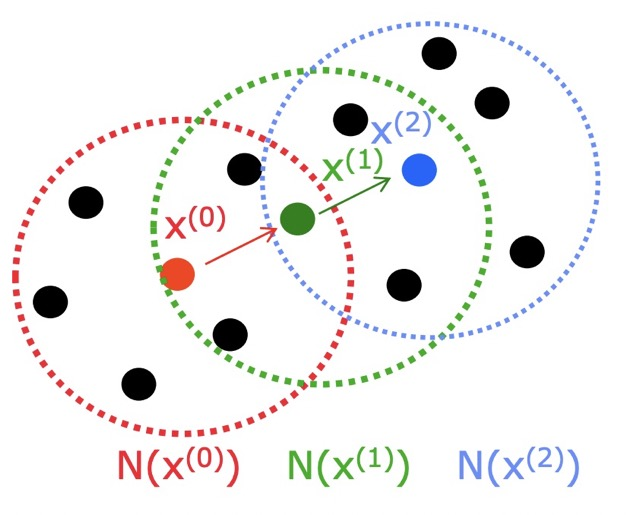
\includegraphics[scale=0.3]{localse.jpeg}
\caption{Local search} 
\label{localse}
\end{figure}


Avremo allora un problema con f.o:
$$\min z = \underline{c}^T\underline{x}$$
s.t.

\begin{itemize}
    \item $\underline{\underline{A}}\ \underline{x} \leq \underline{b}$
    \item $\underline{x} \geq 0$
    \item $\underline{x}$ integer
    \item $\underline{x} \in N(\underline{x}^{(0)})$
\end{itemize}

trovando così una soluzione $\underline{x}^{(1)}$ nell'intorno di $\underline{x}^{(0)}$, ecc ecc...

Sarà un algoritmo di \hl{discesa se minimizziamo} e di \hl{ascesa se massimizziamo}, ma entrambi si \hl{fermeranno in un ottimo locale}.


\begin{figure}[H]
\centering
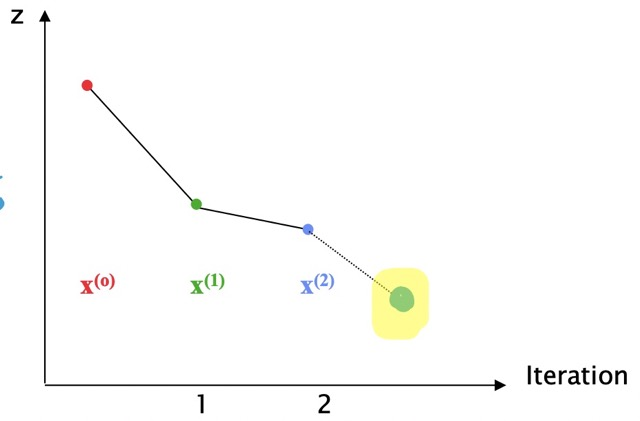
\includegraphics[scale=0.3]{stopsol.jpeg}
\caption{Esempio di ottimo locale} 
\label{stopsol}
\end{figure}


In questo caso un problema:

\begin{itemize}
    \item concavo: avrà un ottimo locale di \textbf{scarsa qualità}
    \item convesso: avrà un ottimo \textbf{uguale a quello globale}
\end{itemize}

Lo \hl{pseudocodice} nel caso di minimizzazione è:

\begin{itemize}
    \item[] INPUT: $\underline{x}^{(0)}$
    \item[] OUTPUT: $\underline{x}^{(k)}$
    \item[] $k = 0$
    \item[] repeat:
    \begin{itemize}
        \item[] solve $(P) + \text{constraint}\ \ \ \forall\ \ \ \underline{x}\in N(\underline{x}^{(k)})$
        \item[] let $\underline{x}^{(k+1)}$ be the optimal solution
        \item[] $k=k+1$
    \end{itemize}
    \item[] until: $z(x^{(k)})<z(x^{(k-1)})$
\end{itemize}

Riprendendo il problema del TSP dovremo \hl{definire un introno} sui punti:


\begin{figure}[H]
\centering
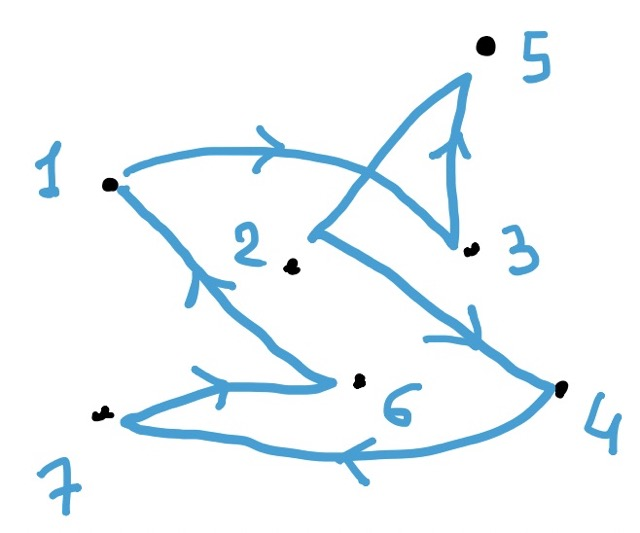
\includegraphics[scale=0.2]{intorno.jpeg}
\caption{Problema del TSP} 
\label{intorno}
\end{figure}


Dobbiamo \hl{definire una perturbazione della soluzione} quindi usiamo un approccio \hl{destroy and repair}:

\begin{enumerate}
    \item \hl{destroy}: \textbf{cancellare 2 archi} come $x_{13}$, $x_{25}$, creando una \hl{soluzione disconnessa} con punti $(1, 6, 7, 4, 2)$ e una con $(3, 5)$
    \item \hl{repair}: \textbf{creo una giunzione più efficiente} tra i due segmenti con $x_{15}$, $x_{23}$
\end{enumerate}

Questo potrebbe portare ad una \hl{variazione di costo}:
$$\text{var. costo } = \text{ archi aggiunti } - \text{archi tolti}$$
$$\Delta z = c_{15} + c_{23} - c_{13} - c_{25}$$


\begin{figure}[H]
\centering
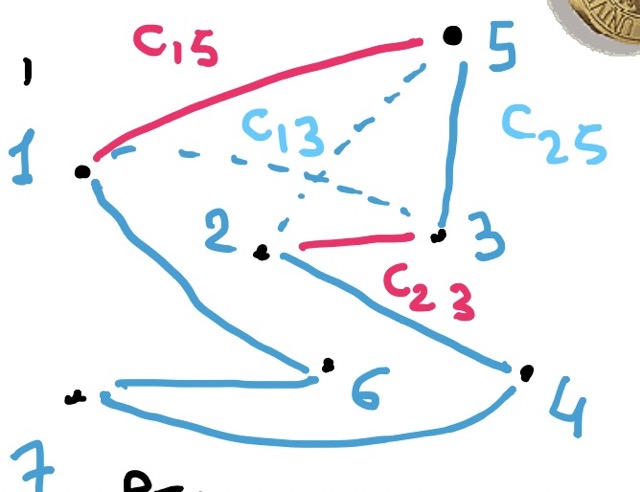
\includegraphics[scale=0.2]{intott.jpeg}
\caption{Ottimizzazione del problema TSP} 
\label{intott}
\end{figure}


L'intorno sarabbe l'\hl{insieme delle soluzioni ottenute dopo il dele and repair}. Quanto troviamo $\Delta z = 0$ ci fermiamo.


% Local branching
\subsection{Local branching}

Se troviamo un \hl{problema a grandi dimensioni} con \hl{variabili binarie}:
$$x1, ..., \in <0, 1>$$

Essendo un problema che \hl{richiederebbe una quantita' elevata di tempo}definiamo un \hl{intorno di un soluzione}. Volendolo dare in pasto ad un solver dobbiamo prima tradurre il vincolo $N(\underline{x}^{(k)})$  in forma di disequazione lineare, \hl{usando la distanza di Hamming} (conto i bit diveri tra due stringhe):

$$\underline{x}^{(k)} = (0,1,1,0,1,1)$$
$$\underline{x} = (1,1,1,0,0,1)$$

con distanza di Hamming: $d(\underline{x}, x^{(j)}) = 2 \text{bits}$.

Allora \hl{data una soluzione $\underline{x}^{(k)}$} avremo che:
$$\underline{x}\in N(\underline{x}^{(k)})\Leftrightarrow d(\underline{x}, \underline{x}^{(k)})\leq m$$

allora dovremo \hl{delle soluzioni $\leq m$}. La \hl{distanza di Hamming tra $\underline{x}$ e $\underline{x}^{(k)}$} sarà:
$$\sum_{j=1,...,n:x_j^{(k)}=0} x_j + \sum_{j=1,...,n:x_j^{(k)}=1} 1-x_j \leq m$$

o ancora meglio con: $\underline{x}k = (0, 1, 1, 0, 1, 1)$ \hl{possiamo contarli con}:
$$x_1 + (1-x_2) + (1-x_3) + x_4 + (1-x_5) + (1-x_6) \leq m$$

\newpage
\section{Multiperiod Lot Sizing model}

% Introduzione
\subsection{Introduzione}
\hl{Discretiziamo il tempo} e quindi divido la pianificazione in \hl{slot di tempo} esistenti come ore, settimane, mesi. Avremo allora una \hl{domanda $d_t$} che fa rferimento al \hl{periodo $t=1,...,T$} con $T$ lunghezza dell'orizzonte di pianificazione.


\begin{figure}[H]
\centering
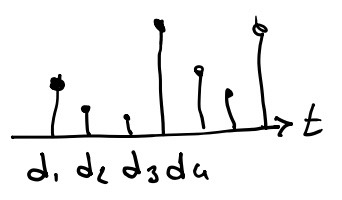
\includegraphics[scale=0.2]{discrettemp.jpeg}
\caption{Discretizzazione del tempo} 
\label{discrettemp}
\end{figure}


Dobbiamo definire:

\begin{enumerate}
    \item varaibili generali:
    \begin{itemize}
        \item \hl{$f_t$}: \textbf{costi fissi di produzione}, potrebbero dipendere dal periodo ma \textbf{non dipendono dalla quantità prodotta} (es: gas, elettricità)
        \item \hl{$c_t$}: \textbf{costi variabili} per la produzione di un prodotto, potrebbe dipendere dal periodo (es: vagetali)
        \item \hl{$h_t$}: \textbf{costi di stockaggio} per un periodo $t$
        \item \hl{Q}: \textbf{capacità di magazzino}
    \end{itemize}

    \item variabili decisionali:
    \begin{itemize}
        \item \hl{$y_t$}: \textbf{variabili di accenzione}
            $$y_t =
            \begin{cases} 
                = 1 \text{se è acceso} \\ 
                = 0 \text{se è spento}
            \end{cases}
            $$

        \item \hl{$x_t$}: indica la \textbf{produzione nel periodo $t$}
        \item \hl{$I_t$}: indica il \textbf{livello di scorte nel periodo $t$}
    \end{itemize}

    \item \hl{funzione obiettivo}:
        $$z = \text{ costi fissi } + \text{ costi variabili } + \text{ costi di inventario }$$
        $$z = \sum_{t=1}^T f_t y_t + \sum_{t=1}^T c_t x_t + \sum_{t=1}^T h_tI_t$$

    \item vincoli:
    \begin{itemize}
        \item \hl{di conservazione delle scorte}: cioè il livello di scorte a fino al periodo precedente e la merce prodotta, togliendo ciò che diamo al mercato:
            $$I_{t-1} + x_t + -d_t = I_t$$
        \item \hl{di capacita'}: dove \textbf{il livello di scorte non deve superare la capacità di magazzino}
            $$I_t \leq Q$$
        \item \hl{lega $x_t$ cno $y_t$}: \textbf{lega accenzione e spegnimento} dei macchinari
            $$x_t \leq (\sum_{i=t}^T) d_i\ \ \ \forall\ \ \ t=1,..,T$$

            essendo $y_t$ binaria, avremo:
            $$y_t =
            \begin{cases} 
                = 1 \to x_t\leq \sum_{i=t}^T d_i  \\ 
                = 0 \to x_t\leq 0\to x_t=0
            \end{cases}
            $$
        \item \hl{sull'inventario}: $I_0, I_T = 0$
        
    \end{itemize}
\end{enumerate}


% Aggiornamento il Beer Game - Backlog
\subsection{Aggiornamento Beer Game - Backlog}

In un problema reale \hl{non sono certo di soddisfare la domanda}, infatti si potrebbe andare \hl{sotto scorta} per cercare di soddisfarla con un \hl{incremento del costo}.
Il \hl{livello delle scorte si divide in una parte positiva ed una negativa}:  
$$I_t = I_t^+ -I_t^- \leq \geq 0$$

con $I_t^+$ livello di inventario e $I_t^-$ backlog.

avremo allora:
\begin{enumerate}
    \item \hl{funzione obiettivo}: 
        $$z = \sum_{t=1}^T f_t y_t + \sum_{t=1}^T c_t x_t + \sum_{t=1}^T h_tI_t^+ + \sum_{t=1}^T b_tI_t^-$$
    \item vincoli:
    \begin{itemize}
        \item \hl{di conservazione delle scorte}:
            $$I_{t-1}^+ - I_{t-1}^- + x_t - d_t = I_{t-1}^+ - I_{t-1}^-\ \ \ \forall\ \ \ t=1,...,T$$
        \item \hl{di capacita'}:
            $$I_t^+ \leq Q$$
        \item \hl{lega $x_t$ cno $y_t$}:
            $$x_t \leq (\sum_{i=t}^T) d_i\ \ \ \forall\ \ \ t=1,..,T$$
    \end{itemize}
\end{enumerate}


% Aggiornamento il Beer Game - Lead time 
\subsection{Aggiornamento Beer Game - Lead time $l\in\{0,1,2,...\}$}

Durante il \hl{periodo di arrivo degli ordini} le prime $l$ settimate non posso sperare di ricevere rifornimenti, infatti \hl{arrivera' nel periodo $t+l$}. Abbiamo i vincoli:

\begin{itemize}
    \item prime $l$ settimane: 
        $$I_{t-1}^+ - I_{t-1}^- - d_t = I_{t-1}^+ - I_{t-1}^-\ \ \ \forall\ \ \ t=1,...,l$$
    \item le altre settimane:
        $$I_{t-1}^+ - I_{t-1}^- + x_{t-l} - d_t = I_{t-1}^+ - I_{t-1}^-\ \ \ \forall\ \ \ t=l+1,...,T$$
\end{itemize}

\newpage
\section{Network Flow Model}


% Introduzione
\subsection{Introduzione}
dove abbimao un grafo  con dei sui parametri che assieme formano un network. dobbiamo allora capire con=me un flusso di dati transitra nellarete.
primo porblema che vediamo
PROBLEMA DI FLUSSO A COSTO MINIMO:

ha la varainte lineare
variante single commodity


in questa classe di problemi abbiamo un grafo G(V, A)
con v vertici e A archi

img


inq uestso caso ogni vetice $i \in V$ o generea o assorbe un flusso di materiali, dati, ecc...

parametro per i nodi:
questo $\forall i \in V: d_i$
> 0 per i = sorgente (souce)
= 0 per i = transito
< 0 per i = pozzo (sink)


se d_i > 0 indica un afornitura
< 0 indica una domanda

caristiche:
single commodity: flusso omogeneo
multiple comodity: varie tipologie di flusso 


parametri per gli archi
prendo un parametro c_{ij} cioe un arco che colega i nodi i e j. c_{ij} = costo (di traspost) unitario (per unita di flusso)
altro paramentro q_{ij}: capacita massima (qunato flusso puo transitrar da i a j)


decisione da prendere: allocaizone del flusso, cioe qunto flusso deve transitare su ogni arco
le varaibili saranno: x_{ij} >= 0 fluso che transita da i a j per unita di tempo


affinche si possa avere una soluzione ammissibile una condizione necessaria è che se sommiamo su utti i vertici le quntita d_i devo avere 0:
$$\sum_{i\in V} d_i = 0$$

quindi non sara sufficiente per via delle capacita degli archi



misure di prestazione della f.o.:
vigliamo allora minimizzare il costo totale di trasporto su tutti gli archi:
$$\min \sum_{(i,j)\in A} c_{ij} x_{ij}$$

notaione epr definire un insieme di vincoli:
dato uun nodo i al quale abbiamo archi uscenti ed entranti allora tutti li archi entranti associamo un insieme $\delta^-(i)$ per quellio uscenti: $\delta^+(i)$


definiiamo allora i vincoli, dobbiamo tenere in conto dei vincoli di conservazione del flusso: cioe che dtutto quello cheentra nel nodo deve uscirci:
$$\sum_{(i,j)\in\delta^+(i)} x_{ij} - \sum_{(j,i)\in\delta^-(i)} x_{ji} = d_i\ \ \ \forall\ \ \ i\in V$$

altri vincoli per avere una soluzione ammissibile abbiamo ance dei vincoli di capacita: avremo un vincolo associato ad ogni arco:
$$x_{ij} \leq q_{ij}\ \  \forall\ \ \ i,j\in A$$

vincoli di non negativita:
$$x_{ij} \geq 0 (\geq l_i)\ \ \ \forall\ \ \ i,j\in A$$

dove l_i quantita minimia in caso di evenienza

la formulazione compatta dice:
$$\min z=\sum_{(i,j)\in A} c_{ij} x_{ij}$$
s.t
- $\sum_{(i,j)\in\delta^+(i)} x_{ij} - \sum_{(j,i)\in\delta^-(i)} x_{ji} = d_i\ \ \ \forall\ \ \ i\in V$
- $x_{ij} \leq q_{ij}\ \  \forall\ \ \ i,j\in A$
- $x_{ij} \geq 0 (\geq l_i)\ \ \ \forall\ \ \ i,j\in A$

formulaizone estesa:
in una topologia di rete cone questa:

img

ad ognmi arco indico c_ij e q_ij e per ogni nodo d_i

allora la fomulazione estesa è: (prendendo il parametro del costo)
$$\min z = 2x_{12} + 5x_{13} + 3x_{23} +3x_{24} + 3_{x32} + 4x_34} + 3x_{42}
s.t
per i = 1: $x_{12} + x_{13} = 10$
per i = 2: $x_23 + x_{24} - x_{12} - x_{42} - x_{32} = 0$
per i = 3: $x_{32} +x_{34} - x_{13} - x_{23} = -3$
per i = 4: $x_42} - x_{24} - x_{34} = -7$

guardando la capacita scriviamo anche:
$x_{12} \leq 8$
$x_{13} \leq 2$
$x_{23} \leq 4$
$x_{24} \leq 7$
$x_{32} \leq 4$
$x_{34} \leq 5$
$x_{42} \leq 7$

$x_{12}, $x_{13}, x_{23}, x_{24}, x_{32}, x_{34}, x_{42} \geq 0$



se un instanza del problema è ammissiibile, cioe se lo sono i dati del problema, allora:
- puo esistere una soluzione ottima
- puo esere unbounded se esiste qualeche arco (i, j) \in A con costo negatico c_{ij} < 0

img

poiche il costo totale negativo nel loop 2,4,5 allora abbiamo:
$$x_{12} = 1, x_{23} = 1, x_{24} = x_{45} = x_{52} = + \infty$$

siuponendo capacita infinita

importante condiione è quella di interezza: dice che se i dati d_i e le capacita q_{ij} sono interi, allora esiste una soluizone ottima non unbounded che è anche esse interacioe x_{ij \in N_0}, cioe i flussi ottimali sono interi.


abbiamo dei casi speciali del problema di flusso a socoto minimo:
- problem a di trasprto (rtansportation problem)
- prob di assegnamento (assignment problem)
- problema di cammino piu breve/rapido (shortesr/quickest path)
- problema di massimo flusso (aximum flow problem)




PROBLEMA DI TRASPORTO:
consideriamo la variante di simple commodity( supponiamo di avere un grafo diaprtito dove l'insieme dei vertici è composto da due insiemi disgiunti: sorgenti (fino a m) e pozzi (fino a n). ad ogni soegente è associata un s_1, .., s_m \geq 0 che definiscono la fornitura e ai pozzi invece abbiamo una qunatita b_1, ..., b_m che rappresenta la domanda. tra questi vertici nei due insiemi abbiamo na coppia di sorgente-pozzo e per ogni arco ij è associato un costo cij (costo i trasporto per unita di flusso)

img

allora il grafo G è dato da: G = (V=v_1 \cup V_2, A) con V_1 \cap V_2 = insieme vuoto e viene detto grafo rbipartito ed è questo problemaun caso speciale del problema di flusso a caso minimo, nel qule abbiamo che:
- non abbiamo vincoli di capacita
- non abbiamo nodi di transito

il problema sara allora ammissiible se:
$$\sum_{i\in V_1} s_i = \sum_{i\in V_2} b_i$$

allora le varaibili abbiamo che:
$$x_{ij}, i\inV_1, j\in V_2$$ che indica qunate unuta di flusso ("merce") vengono gtraspostate da i a j


l'obiettivo è minimizzare al f.o. quindi la misura di prestazione sara: $\min z = \sum_{(i,j)\in A}\sum_{j\inV_2} c_{ij}x_{ij}$ alora minimizziamko il costo totale.

vincoli:
$$\sum_{j\in V_2} x_{ij} = s_i\ \ \ \forall\ \ \ i\in V_1$$ per ongi vertice sorgente
$$\sum_{i\in V_1} x_{ij} = b_i\ \  \\forall\ \ \ j\in V_2$$ per ongi vertice pozzo
$$x_{ij} \geq 0\ \ \ \forall\ \ \ i\in V_1, j\in v_2$$



PROBLEMA DI ASSEGNAMENTO LINAERE:
abbiamo sempre un siseme di vertici diviso in due grupi: n risorse e n tasks
obiettvo assengare le risorse ai tasks

img

assegnamo iun costo sll'arco ij con c_{ij}.

ad una risorsa possiamo associare un solo task.
es: magazzini (impianti) automatizzati: n = 4 con n risorse = ABV (automated guided vehicle)
abbiamo dei task da compiere come lo spostamente di un veicolo da un punto ad un altro

img

avremo allora i costi di oni veicolo per spostarsi allinizio del task
costi = tempo di viaggio dal puno di prelievo al punto di inizio

quindi questa tipologi a di problemi è un acso speciale del prtiblema di trasposto dove cambia solo che:
- m= n
- s_i = 1 \forall i
- b_i = 1 \forall j


le variabili saranno allora:
x_{ij} = 1 se la rosorsa i è aasegnata ad un task j
= 0 altrimenti

vorremo allora minimizzare la f.o.: $\min z = \sum_{i=1}^n\sum_{j=1}^n c_{ij} x_{ij}$
s.t.
- $\sum_{j=1}^n x_{ij} = 1\ \ \ \forall\ \ \i=1,...,n$ cioe ogni risrosa deve essere assegna ad un solo task
- $\sun_{i=1}^n x_{ij} = 1\ \ \ \forall\ \ \ j=1,...,n$ cioe ongi task deve essere assegnato ad una sola risorsa

dato che s_i = 1 con i = 1,...,n e b_j = 1 con j=1,...,n

possiamo imporre che x_{ij} \geq 0 impedendo che la variabile sia <= 0 qusto grazie all;interezza dei dati e ai vincoli qui sopra che impediscono che le varaibili assumano valore > 1 quidni potremo avere con valore 0 o 1.













\end{document}
%%%%%%%%%%%%%%%%%%%%%%%%%%%%%%%%
%%%%%% FINE DEL DOCUMENTO %%%%%%
%%%%%%%%%%%%%%%%%%%%%%%%%%%%%%%%




